\documentclass[a4paper,12pt]{book}
\usepackage[english]{babel}
\usepackage[utf8]{inputenc}
\usepackage{graphicx}
\usepackage{menukeys}
\usepackage{amsmath}
\usepackage{amssymb}
\usepackage[T1]{fontenc}
\usepackage{upquote}
\usepackage{wrapfig}
\usepackage{makeidx}
\usepackage{tikz, pgf}
\usepackage{listing}
\usepackage{fancyvrb}


\usetikzlibrary{backgrounds, positioning, %% Draw Y-chart
snakes, fit,                            %% Draw Y-chart
3d,  arrows, automata, shapes.gates.logic.US,
shapes.gates.logic.IEC, calc, 
circuits.logic.US}
\usepackage{circuitikz}

\newsavebox{\fmbox}
\newenvironment{fmpage}[1]
           {\begin{lrbox}{\fmbox}\begin{minipage}{#1}}
           {\end{minipage}\end{lrbox}\fbox{\usebox{\fmbox}}}

\addto\captionsenglish{\renewcommand{\figurename}{Listing}}

\makeindex

\title{An introduction to Low Level Lisp\\
{\normalsize (Content not checked for grammar and spelling errors)}}
\author{Eduardo Costa \and Vernon Sipple}
\date{}

\begin{document}
\maketitle
\thispagestyle{empty}

\mainmatter

\chapter{Emacs commands}
In the next chapter, you will learn how to install
Emacs. To give you a head start, this chapter
lists the basic commands you need to edit a file.

In the following cheat sheet, \verb|Spc| denotes
the space bar, \verb|C-| is the \keys{Ctrl} prefix, \verb|M-| represents 
the  \keys{Alt} prefix and  $\kappa$ can be any key. 

\paragraph{Basic commands.} \verb|C-|$\kappa$ -- Press and release \keys{Ctrl}
and \keys{$\kappa$} simultaneously
\begin{quote}
 \verb|C-s| then type some text -- search a text.\\
 \verb|C-r| then type some text, -- reverse search.\\
 \verb|C-k| -- kill a line.\\
 $\longleftarrow$ \verb|backspace| -- backspace.\\
 \verb|C-d| -- delete char forward.\\ 
 \verb|C-Spc| then move the cursor -- select a region.\\
 \verb|M-w| -- save selected region into the kill ring. \\
 \verb|C-w| -- kill region.\\
 \verb|C-y| -- insert killed or saved region.\\
 \verb|C-g| -- cancel minibuffer reading.\\
 \verb|C-a| -- go to beginning of line.\\
 \verb|C-e| -- go to end of line.\\
 \verb|C-b| -- move backward one character.\\
 \verb|C-f| -- move forward one character.\\
 \verb|C-n| -- move cursor to the next line.\\
 \verb|C-p| -- move cursor to the previous line.\\
 \verb|C-/| -- undo. \\
 \verb|C-v| -- forward page.\\
 \keys{INS} -- toggle overwrite mode.\\
 \keys{$\leftarrow$} \keys{$\rightarrow$} \keys{$\uparrow$} \keys{$\downarrow$} -- arrows move cursor.\\
\end{quote}
\paragraph{Control-x commands.} \verb|C-x C-|$\kappa$ -- Keep \keys{Ctrl}
down and press \keys{x} and  \keys{$\kappa$}
\begin{quote}
\verb|C-x C-f| -- open a file into a new buffer.\\
\verb|C-x C-w| -- write file with new name.\\
\verb|C-x C-s| -- save file.\\
\verb|C-x C-c| -- exit emacs.\\
\verb|C-x i| -- insert file at the cursor.\\
\verb|C-h c| -- describes a key stroke.\\
\verb|M-x | {\bf shell} --  shell command. After \verb|M-x|,
if one types \verb|shell| at the prompt, the computer
will enter the shell of an ANSI terminal.
It is possible to use many other command
just like the \verb|shell| given as example.
\end{quote}



\paragraph{Window commands.} One can have more
than one window on the screen. Below, you will
find commands that cope with this situation.
\begin{itemize}
\item \verb|C-x |$\kappa$ -- Press and release \keys{Ctrl}
and \keys{x} together, then press \keys{$\kappa$} 
\begin{quote}
\verb|C-x b| -- switch to buffer. User arrows to choose the buffer\\
\verb|C-x C-b| -- list buffers.\\
\verb|C-x k| -- kill current buffer.\\
\verb|C-x =| -- char at cursor position.\\
\verb|C-x 2| -- split window into cursor window and other window.\\
\verb|C-x o| -- jump to the other window.\\
\verb|C-x 1| -- close the other window.\\
\verb|C-x 0| -- close the cursor window.
\end{quote}
\item \verb|Esc| $\kappa$ -- Press and release the \keys{Esc} key,
then press the \keys{$\kappa$} key.
\begin{quote}
\verb|Esc >| -- go to the end of buffer.\\
\verb|Esc <| -- go to the beginning of buffer.\\ 
\verb|Esc f| -- word forward.\\
\verb|Esc b| -- word backward.\\
\end{quote}
\item \verb|M|-$\kappa$ -- Keep the \keys{Alt} key
down and press the \keys{$\kappa$} key.
\begin{quote}
\verb|M-b| -- move backward one word.\\
\verb|M-f| -- move forward one word.\\
\verb|M-g| {\bf goto-line} -- go to the line given in the minibuffer.\\
\verb|C-x| $\rightarrow$-- activate the next buffer.\\
\verb|C-x| $\leftarrow$ -- go to previous buffer.\\
\verb|C-Spc C-Spc| -- set a return position.\\
\verb|C-u C-Spc| -- go to return position after a long jump.
\end{quote}
\end{itemize}

\paragraph{Query replace.} If you press
\keys{Esc}\keys{x} {\bf replace-string}
RETURN, type the search string and
press RETURN again, then provide the
replacement string, computer enters
in the query replace mode. First, emacs
prompts for the text snippet S
that you want to replace. Then it prompts for
the replacement R. When you type the R text and
press the \keys{Enter} key, the cursor jumps to
the first occurence of S, and emacs
asks whether you want to
replace it. If the answer is
\verb|y|, emacs will replace S
with \verb|R| and jump to the next occurence.
If the answer is \verb|n|, emacs will
jump to the next occurrence of S without
performing the replacement.

\paragraph{Go to line.} When you try to compile
code containing errors, the compiler
usually reports the line number where the error occurred.
If you press \keys{Esc}\keys{x} then {\bf goto-line},
emacs prompts for a line number. As soon as you
type the number and press the \keys{Enter}
key, the cursor jumps to the given line.

In order to know the position of the cursor,
press the \verb|C-x =| command,
and emacs gives information concerning
the character under the
cursor, the corresponding code, the line,
and the character position in the text.

\paragraph{List bindings.} If you press
the \verb|C-h b| command,
the computer lists all key bindings.
On the other hand, the \verb|C-h c| command
prompts you for a key sequence
and describes it.


\paragraph{Nia Vardalos.}
In order to get acquainted with editing,
let us accompany the Canadian programmer Nia
Vardalos, while she explores emacs.

When text is needed for carrying out a command,
it is read from the minibuffer, a one line
window at the bottom of the screen. For instance, 
if Nia presses \verb|C-s| for finding a text, 
the text is read from the minibuffer. After
localizing the text, Nia presses \verb|Enter|
to interrupt the search. For abandoning an ongoing
command, she may press \verb|C-g|. To search the
same text again, Nia presses \verb|C-s C-s|
twice.

To transport a region from one place to another,
Nia presses \verb|C-Spc| to start
 the selection process 
 and move the cursor to select the region. 
 Then she presses \verb|C-w| to
kill her selection. Finally, she moves
the cursor to the insertion place,
and presses the \verb|C-y| shortcut.
To copy a region, Nia presses \verb|C-Spc| and moves
the cursor to select the region.
Then she presses \verb|M-w| to save the selection
into the kill ring. Finally,
she takes the cursor to the destination where the
copy is to be inserted and
issues the \verb|C-y| command.

Nia noticed that there are two equivalent ways to
issue an \verb|M-|$\kappa$ command. She can
press and release the \keys{Esc} key, then
strike the  $\kappa$ key. Alternatively, she
can keep the \keys{Alt} key down and press
the \keys{$\kappa$} key.

\paragraph{Calculations with Lisp.} Emacs
offers a Lisp dialect to perform calculations
and text processing. Let us assume that you
want to find how many students graduate
from medical schools in California. You
press \keys{Esc}\keys{x} and type {\bf ielm}
at the {\bf M-x} prompt, and emacs
will place you in a Lisp chat box.
\begin{quote}
\verb|ELISP> (+ 190 180 170 160 120 100 100 90)|\keys{Enter}
\end{quote}
In the above expression, the first thing after
the open parenthesis is the \verb|+| sum
operation identifier. After the name of
the operation, there is a list of
the arguments to be added together.
As soon as Nia presses the \keys{Enter} key,
emacs shows the result of the addition:
\begin{quote}
\verb|1110|
\end{quote}
The rule that worked for 
the $\verb|(+ | x_1\;x_2\ldots\verb|)|$
sum operation also works for the 
other arithmetic function too.
\begin{itemize}
  \item{Multiplication} is performed
by the \verb|*| operation.
\begin{quote}
\keys{Esc}\keys{;}\\
\verb|ELISP> (* 1 2 3 4 5)|\keys{Enter}\\
120
\end{quote}
\item{Division} is obtained through the \verb|/| operation.
\begin{quote}
\keys{Esc}\keys{;}\\
\verb|ELISG> (* 1 2 4)|\keys{Enter}\\
0.125
\end{quote}
The above operation performed the chain
division \verb|1/2/3|.
\item{Subtraction} has the syntax shown below.
\begin{quote}
\keys{Esc}\keys{;}\\
\verb|ELISP> (- 1 2 4)|\keys{Enter}\\
-5
\end{quote}
\item Mixed operations. One can nest subexpressions
  within an outer expression. For instance,
  to get the average student number graduating
  from medical school in California, one can
  calculate the expression:
\begin{quote}
\keys{Esc}\keys{;}\\
\verb|ELISP> (/ (+ 190 180 170 160 120 100 100 90) 8)|\keys{Enter}
\end{quote}

\end{itemize}

\paragraph{Command execution.} When you press 
shortcut keys, femto emacs call a command written in
C or in Lisp. You can get a complete list of all
emacs commands by pressing the 
\verb|C-h|\keys{$b$} shortcut.

There are commands that are not associated to
 shortcut keys. 
For instance, the \verb|goto-line| command
is obtained by pressing \verb|M-x| then typing
{\bf goto-line} at the minibuffer prompt.
Below you will find a fairly complete list
of emacs commands.

\begin{verbatim}
backspace        backspace
C-a              beginning-of-line
C-b              backward-character
C-d              forward-delete-char
C-e              end-of-line
C-f              forward-character
C-k              kill-line
C-n              next-line
C-p              previous-line
C-r              search-backward
C-space          set-mark
C-s              search-forward
C-/              undo
C-w              kill-region
C-x 1            delete-other-windows
C-x 2            split-window
C-x C-b          list-buffers
C-x C-c          exit
C-x C-f          find-file
C-x C-<Right>    next-buffer
C-x C-<Left>     previous-buffer
C-x C-s          save-buffer
C-x =            what-cursor-position
C-x C-w          write-file
C-h c            describe-key
C-x i            insert-file
C-x k            kill-buffer
C-x o            other-window
M-x shell        shell-command
C-y              yank
<down>           next-line

esc b            backward-word
esc <            beginning-of-buffer
esc w            copy-region
esc d            kill-word
esc >            end-of-buffer
esc f            forward-word
M-x goto-line    goto-line

C-h b            list-bindings
C-Spc            set-mark
        
esc @            mark-word
esc <            beginning-of-buffer

esc w            copy-region
esc x            execute-command
home             beginning-of-line
INS              toggle-overwrite-mode
<left>           backward-character

<right>          forward-character
<up>             previous-line
\end{verbatim}

\chapter{Installation}  
A text editor, like Emacs, has three components:
\begin{enumerate}
\item A frontend that inserts characters into a buffer.
A buffer is a memory region with an image of a
text file. One can see the buffer as a representation
of a scratch pad. As such, the frontend provides tools to
insert keystrokes at the  point indicated by 
a movable cursor.
\item Editing operations that save buffers
as files, delete and insert text, move the
cursor around, copy items from one place to another, etc.
\item A scripting language for customizing the editor.
\end{enumerate}

There is a large choice of frontends. Some frontends 
work with a raster graphics image, which  is a dot matrix 
data structure that represents a grid of pixels. 
There are also frontends that are specialized in
showing letters and other characters via an appropriate
display media. The latter sort of frontend is called
text-based user interfaces, while the former is called
graphical user interface, or GUI for short.

Text-based user interfaces are more
confortable on the eyes, since they  provide
sharper and crisp alphabetical letters.
On the other hand, GUI allows for font 
customization. At present,
emacs offers both ncurses, which
is a text-based user interface, and also GUI.
Search the Internet for a distribution that
works in your computer, download and install it
according to the instructions of the vendor.

You will also need Bigloo. Search the Internet
for Bigloo scheme, download and install it, as
you did in the case of Emacs.

Both Bigloo and Emacs, like any piece of sofware,
are quite difficult  to install. It is possible
that you will not find a binary distribution.
In this case, you will need to build the package,
before performing the installation. If computer
science is not your thing, ask for help. In the
United States, in the neighborhood of large
universities, it is quite easy to find very capable
students that will install Bigloo and Emacs for food.


\includegraphics[scale=0.6]{figs-prefix/download.png}


\section{Ready}
You are now ready for action!


\includegraphics{figs-prefix/readyforaction.jpg}

It seems that people prefer money to sex.
After all, almost everybody says no to
sex on one occasion or another.
But I have never seen a single
person refusing money. Therefore, let us
start this tutorial talking about money.


\index{Arithmetic!Elemetary School}  
\begin{wrapfigure}[10]{i}{5cm}
\renewcommand\figurename{Fig.}

\includegraphics[scale=0.5]{figs-prefix/firemen.png}
\caption{Running total}
\end{wrapfigure}

If one wants to calculate a running
total of bank deposits, she will make
a column of numbers and perform the
addition.


What I mean to say is that, if you
need to perform the addition
$8 + 26 + 85 + 3$ with pencil and paper,
you will probably stack the numbers the
same way you did before taking pre-algebra
classes in highschool:
\begin{quote}
\begin{tabular}{p{0.5cm}p{1cm}}
+ &\verb|  8|\\
&\verb| 26|\\
&\verb| 85|\\
&\verb|  3|\\
\hline
&\verb|122|
\end{tabular}
\end{quote}
Subtraction is not treated differently:
\begin{quote}
\begin{tabular}{p{0.5cm}p{1.5cm}}
\Large\bf -&   358\\
&   216\\
\hline
& 142
\end{tabular}
\end{quote}

This chapter contains an introduction to
the Cambridge prefix notation, 
which is slightly different from the one you
learned in elementary school: The operation
and its arguments are put between parentheses.
In doing so, one does not need to draw a line
under the bottom number, as you can see below:
\begin{quote}
\begin{tabular}{p{0.5cm}p{1cm}}
(+ &\verb|  8|\\
&\verb| 26|\\
&\verb| 85|\\
&\verb|  3|)\\
&\verb|122|
\end{tabular}
\end{quote}
The Cambridge prefix notation can be applied
to any operation, not only to the four arithmetic
functions. 

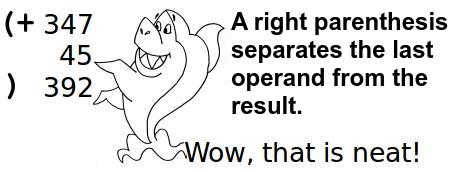
\includegraphics{figs-prefix/neatsum.jpg}

\section{Cambridge prefix notation}
\index{Prefix notation}
\index{Prefix notation!Cambridge}
Let us summarize what we have learned
until now. In pre-algebra, students
learn to place arithmetic operators (+, -, × and ÷)
between their operands; e.g. 347+45.
However, when doing additions and subtractions
on paper, they stack the operands.

%% 
\includegraphics{figs-prefix/stackshark.jpg}


Lisp programmers put operation and operands
between parentheses. The right parenthesis
separate the operands from the result,
instead of drawing a line under the last operand.
This syntax is used both by Bigloo, Emacs
Lisp and WebAssembly. It was discovered by a
logician whose name is Jan Łukasiewicz, for this
reason it is called Polish prefix notation, after
Łukasiewicz nationality.

The Polish notation has an interesting mathematical
property: It is the simplest language that is expressive
enough to represent mathematical and logical well
formed formulas. Let us see the consequences of this
mathematical syntax.

\subsection{Lisp and Mathematics}

Computer languages have, in general, a very complex syntax.
A  Python programmer, for instance, must learn many syntactical
variants for calling up an expression. The function that
calculates the logarithm has a prefix notation, while arithmetic
operations obey infix syntax rules.

\begin{verbatim}
>>> math.log(3,4)
0.7924812503605781
>>> (3+4)*(5+6+7)*8
1008
\end{verbatim}

Instead of accepting an arbitrary syntax, Lisp  adopted
symbolic expressions, which evolved from a mathematical
notation proposed by \L ukasiewicz in 1920. In mathematics,
basic constructions and transformation rules are kept
to a minimum. This {\sc lex parsimoni\ae} has many
consequences. The first being that few rules can classify
all symbolic expressions:

\begin{enumerate}
\item Numerals have traditional notation: 3, 3.1416, -8, etc. 
\item Symbols are  sequences of characters that cannot be
  interpreted as numbers and do not contain brackets:
  \verb|sin|, \verb|x|, \verb|y|, \verb|*ops*|, etc.
\item Quoted lists such as \verb|'(a b e)| represent
  sequences of objects.
\item Unquoted  lists such as \verb|(log 8 2)| denote
  function calls.
\item Abstractions such as \verb|(lambda(x y) (log (abs x) y))|
  define   functions. The sequence of symbols \verb|(x y)| is called
  a binding list, and the expression \verb|(log (abs x) y)| is the
  body of the abstraction.
\end{enumerate}

Any variable that appears in the binding list is said to be bound.
Free variables occur in the body of the abstraction but not in the
binding list.

Another consequence of its mathematical foundations is that Lisp
has a clear and simple semantics. The rules of computation are
based on a Mathematical system called the Lambda Calculus.

\begin{description}
\item[$\alpha$-conversion] Changing the name of a bound variable
  produces equivalent expressions. Therefore,  $(\lambda(x) x)$
  and $(\lambda(y) y)$ are equivalent.
\item[$\beta$-reduction] $((\lambda(x) E) v)$ can be reduced
  to $E[x := v]$.
\end{description}

Lisp has a Read Eval Print Loop (REPL) that performs
$\beta$-reduction over symbolic expressions in order to
simplify their forms. In the $\beta$-reduction process,
the first element of a list can be considered as
a function or a macro.

In Lisp, all functions follow the list syntax, without a single
exception: The first element of the list is the function
identifier, and the other elements are arguments. In order to
start Bigloo Scheme, a dialect of Lisp, execute the command
\verb|M-x shell| from Emacs (keep the \keys{Alt} down and
press the \keys{A} key, then type {\bf shell}). From the
terminal call the Bigloo interpreter, as shown below.

\begin{verbatim}
~/LLLdocs$ bigloo -s

1:=> (expt 3 4)
81
1:=> (* (+ 3 4) (+ 5 6 7) 8)
1008
1:=> (exit)
~/LLLdocs$ 
\end{verbatim}

One immediate advantage of its mathematical foundations is that
Lisp is unlikely to become obsolete. This means that one may
expect that a language like Python or Fortran to suffer changes
without backward compatibility. One can even expect that Python
or Fortran would be phased out. However, Lisp code written many
decades ago can be easily run in a modern computer. Besides this,
since Lisp does not change, computer scientists can work on Lisp
compilers for many decades, which results in fast and robust code.



\section{Pictures}
Here is the story of a Texan who went on
vacation to a beach in Mexico. While he was
freely dallying with the local beauties,
unbeknowest to him a blackmailer took some
rather incriminating photos.
After a week long gallivanting, the Texan
returns to his ranch in a small town near Austin.
Arriving at his door shortly after is the blackmailer
full of bad intentions.

Unaware of any malice, the Texan allows the so
called photographer to enter and sit in front
of his desk. Without delay, the blackmailer spread
out a number of photos on the desk, along with his
demands: “For the photo in front of the hotel,
that will cost you \$~25320.00. Well, the one
on the beach that's got to be \$~56750.00.
Finally, this definitively I can't let
go for less than \$~136000.00.”

Once finished with his presentation,
the blackmailer snaps up the photos,
and looks to the Texan with a sinister
grin, awaiting his reply.

Delighted with the selection of pics,
the Texan in an ellated voice says:
“I thought I would have no recollection
of my wonderful time. I want 3 copies
of the hotel shot, half a dozen of the beach.
And the last one, I need two copies for myself,
and please, send one to my ex-wife.
Make sure you leave me your contact
details; I might need some more.

\paragraph{Mixed calculations.}
In order to calculate how much the
Texan needs to pay his supposed blackmailer,
his bookkeeper needs to perform the
following operations:
$$3\times 25320+6\times 56750 + 2\times 136000+136000$$
It should be remembered that multiplications
within an expression take priority over additions
and subtractions. The bookkeeper must therefore
calculate the first two products $3\times 25320$
and $6\times 56750$, before performing the first
addition. In the Cambridge prefix notation,
the internal parentheses pass priority over
to the multiplications.

The Texan's bookkeeper started emacs
in order to visit the \verb|finance.scm|
file. The text editor creates a memory
buffer that mirrors the file contents.
By convention, the file and the buffer
have the same name.

Initially, the \verb|finance.scm| buffer
is empty, but the bookkeeper will fill it
with expressions and the corresponding
calculations. Here is how to start the
text editor:
\begin{quote}
\begin{verbatim}
~/wrk/wasm$ emacs -nw
\end{verbatim}
\end{quote}
From emacs, type \verb|M-x shell| command, then
\verb|bigloo -s| to start the interactive
interpreter. Listing~\ref{texan:photos} shows what
an interaction with the Bigloo buffer looks like.

\begin{figure}[!h]
\begin{fmpage}{0.8\textwidth}
  \begin{verbatim}


  \end{verbatim}
\end{fmpage}

\begin{fmpage}{0.8\textwidth}
\verb|1:=>(+  (* 3 25320)|\\
\verb|        (* 6 56750)|\\
\verb|        (* 3 136000) )|\keys{Enter}\\ 
824460
\end{fmpage}

\begin{fmpage}{0.8\textwidth}
\begin{verbatim}
M-x shell 
\end{verbatim}
\end{fmpage}
\caption{The finance.scm buffer}
\label{texan:photos}
\end{figure}


\section{Time value of money}
Suppose that you wanted to buy a \$ 100,000 red Ferrari,
and the forecourt salesperson in his eagerness to
close a deal gives you the following two payment options:  
\begin{itemize}
\item Pay \$ 100,000 now {\bf or}
\item pay the full \$ 100,000 after a three year grace period.
\end{itemize}

I am sure that you would choose to pay the \$ 100,000 after
three years of grace has finished, although you have the
money in a savings account waiting for a business
opportunity. But why is this? After all, you will need
to pay the debt one way or the other. However, if you
keep the money in your power during the grace period,
you can earn a few months of fuel from the interest.

You may not know for sure how much interest you
will earn in three years, but since the salesperson
is not charging you for deferring the payment,
whatever you gain is yours to keep.

Unfortunately for you, the above scenario would
more than probably not happen in real life.
The right to delay payment until some future
date is a merchandise with a price tag,
which {\em is called interest by those who
think it lawful, and usury by those who
do not} (William Blackstone's Commentaries
on the Laws of England). Therefore, unless
the salesperson is your favorite aunt,
the actual offer is like jumping into a tank
full of sharks as in the classic James Bond films.
It requires a little forethought and understanding
of how interest works, before making a decision.
Here is a more realistic real estate sales offer:

\begin{itemize}
\item \$ 100,000 now {\bf or}
\item \$ 115,000 at the end of three years.
\end{itemize}

What to do when facing an increase in price
to cover postponement of payment? The best
policy is to ask your banker how much interest
she is willing to pay you over your
granted grace period.

Since the economy performance is far
from spectacular, your banker offers you
an interest rate of 2.5\%, compound annually.
She explains that compound interest arises
when interest is paid on both the principal
and also on any interest from past years.

\section{Future value}\index{Future Value}

%%
\includegraphics{figs-prefix/piggy.jpg}

The value of money changes with time. Therefore,
the longer you keep control of your money,
the higher its value becomes, as it can earn
interest. Time Value of Money, or TVM for short,
is a concept that conveys the idea that money
available now is worth more than the same
amount in the future.

If you have \$ 100,000.00 in a savings account
now, that amount is called {\em present value},
since it is what your investment would give you,
if you were to spend it today.

Future value of an investment is the amount
you have today plus the interest that your
investment will bring at the end of a
specified period.

The relationship between the present value
and the future value is given by the
following expression:
\begin{equation}
FV= PV\times (1+i)^n
\label{eq:future-value}
\end{equation}
where $FV$ is the future value, $PV$ is the present
value, $i$ is the interest rate divided by 100,
and $n$ is the number of periods.

\begin{figure}[!h]
\begin{fmpage}{0.8\textwidth}
\verb|1:=> (* 100000.00 (expt (+ 1.0 0.025) 3))|\keys{Enter}\\
\verb|107689.06|
\end{fmpage}
\caption{Command from Bigloo interpreter}
\label{future-value}
\end{figure}

In the case of postponing the payment of a \$ 100,000.00 car
for 3 years, at an interest rate of 0.025, the future
value of the money would be 107,689.06; therefore,
I stongly recomend against postponing the payment.

Let us summarize what you have learned until now.
When you open the emacs editor, there is
a one line minibuffer at the bottom of the screen.
If you keep the \keys{Alt} key pressed,
and strike the  \keys{~x~} key, the editor
will prompt you for command. Type {\bf shell}
to open a terminal. Then call the Bigloo interpreter
with \verb|bigloo -s| and type prefix expressions
for the computer to calculate.


\section{Compound interest}

Our Texan decides he needs a break. Thus he walks into
a New York City bank and asks for the loan officer.
He tells a story of how through his doctor's recomendation
he was taking it easy at his property in the south of
France for two whole years and for such a medical
emergency he needs a \$ 10,000.00 loan.

The loan officer said that the interest was a compound 8\%
a year, but the bank would need some collateral for the loan.

“Well, I have a 60 year old car that I like very much.
Of course, I cannot take it with me to France.
Would you accept it as collateral?”

Unsure whether or not the old car was worth the
amount of the loan, the officer summons the bank manager.
The manager inspects the vehicle that was parked on the
street in front of the bank. After a close examination,
he gives a nod of approval: “It’s a Tucker Torpedo.
Give him the loan.”

The Texan quite willingly signed his heirloom over.
An employee then drove the old car into the bank’s
underground garage and parked it. From time to time,
the employee would go, and turn over the engine, to keep
the car in good running condition, and gave it an
occasional waxing just to maintain it in pristine condition.
Two years later the Texan returned, and asked how
much he owed the bank. The loan officer started emacs,
and calculated the total debt as \$ 11,664.00.

\paragraph{Interest Calculation.}
\index{Interest!Compound}
Let us follow the calculation of the value accumulated
in the first year of compound interest at a 8\% rate
over \$ 10,000.00. Press \keys{Ctrl}\keys{~o~} and
enter formula~\ref{eq:future-value} in the minibuffer:
\begin{quote}
\begin{verbatim}
1:=> (* (expt (+ 1.0 0.08) 2) 10000)
11664.000000000002
\end{verbatim}
\end{quote}
Observe that it was necessary to divide the
interest rate by 100, which produces 0.08.

It is possible to define an operation that
calculates formula~\ref{eq:future-value}
given the arguments \verb|fv|, \verb|i|
and \verb|n|. The definition is given
in listing~\ref{Texan:parking}.
Start the editor from a text terminal:
\begin{quote}
\begin{verbatim}
~$ mkdir financing
~$ cd financing
~/financing$ emacs -nw fvalue.scm
\end{verbatim}
\end{quote}
After typing the definition shown
in listing~\ref{Texan:parking},
you must issue the \keys{Ctrl}\keys{~x~}
\keys{Ctrl}\keys{~s~}
command to save the buffer.
In order to do this, keep the
\keys{Ctrl} key pressed down and
hit the \keys{~x~} and
\keys{~s~} keys in sequence.

In order to load the program into
scheme, type \verb|(load "fvalue.scm")|
in the Read Eval Print Loop (REPL) of the interpreter,
as shown in listing~\ref{Texan:parking}. The
interpreter is called REPL because it is
continously reading, evaluating and printing
symbolic expressions (sexpr), that is how
scheme and WebAssembly expressions are called.

In listing~\ref{Texan:parking}, text
between a semicolon and the end of
a line is considered a comment.
Therefore, \verb|;; File: fvalue.scm|
is a comment. Likewise, \verb|;;end define|
is a comment. Comments are ignored by
scheme, and have the simple function of
helping people.

\begin{figure}[!h]\index{define}
\begin{fmpage}{0.8\textwidth}
\begin{verbatim}
;; File: fvalue.scm

(define  (future-value pv i n)
(* (expt (+ (/ i 100.0) 1) n) 
   pv)
);;end define
\end{verbatim}
\end{fmpage}

\begin{fmpage}{0.8\textwidth}
\begin{verbatim}
~/LLLdocs$ bigloo -s

1:=> (load "fvalue.scm")
fvalue.scm
1:=> (future-value 10000 8 2)
11664.000000000002
\end{verbatim}
\end{fmpage}
\caption{Future Value Program}
\label{Texan:parking}
\end{figure}


\section{Mortgage}
A man with horns, legs and tail of a goat,
thick beard, snub nose and pointed ears entered
a real estate agency, and expressed his intention
of closing a deal. People fled in all directions,
thinking that Satan himself was paying them a visit.
Deardry seemed to be the only person who remained
calm. “What a ignorant, narrow minded, prejudiced
lot! I know you are not the devil. You are the
Great God Pan! What can I do for you?”


“I would like to buy a house in London.
I know that the city is made up of 32 Boroughs
and where I buy will make an enormous difference
to price, quality of life, and chances of increase
in capital value of the property.”

“Well, Sir, with our experience you can rest
assured that you will secure your ideal property.
Firstly we must decide on what type of property
fits your needs and where you want to be. You
may consider somewhere like Fulham, Chelsea,
Knightsbridge, Kensington or Mayfair.
I have properties in all these places. ”

“Chelsea! I like the name.”

“Chelsea is arguably one of the best residential
areas in London. It has benefited from it’s close
proximity to the west end of the city and is highly
sought after by overseas buyers looking to be located
in one of the most popular areas in central London.
At the moment, I can offer you a fantastic living
space in a four bedroomed flat situated behind
King's Road. The price is £10,500,000.”


\includegraphics[scale=0.5]{figs-prefix/greatgodpan.jpg}

“I don't have this kind of cash with me right now,
but can get it in a few months of working in a
circus. Meanwhile, can you arrange a mortgage for me? ”

“Yes, Yes I can help arrange mortgages in all 32 Boroughs
of London. Non-residents can have mortgages up to 70\% of
the purchase price. Do you have £3,150,000 pounds for the
down payment? In mortgage agreements, down payment is
the difference between the purchase price of a property
and the mortgage loan amount.”

“I know what down payment is. And yes, I can dispose
of £3,150,000 pounds.”

“A mortgage insurance is required for borrowers with
a down payment of less than 20\% of the home's purchase
price. That is not your case. Therefore, the balance of
the purchase price after the down payment is deducted
is the amount of your mortgage. Let us write a program
in scheme to find out your estimated monthly payment.
The loan amount is £7,350,000 pounds. The interest rate
is 10\% a year. The length of the mortgage is 20 years.
That is the best I can do for you, I am afraid.
You are going to pay £97131.00 pounds a month for
ten years. After that, the balance of your debt
will be zero. But your visit is a surprise!”
The broker exclaimed. “ I never thought I would
ever see a true living god wanting to do property
deals in London.”

With that, Pan replied: “If property prices
were not so high, and interest rate so steep,
we would definitely be up for business more often.”



\paragraph{Loan Amortization.}
Amortization refers to the gradual reduction
of the loan principal through periodic payments.


\includegraphics{figs-prefix/agingshark.jpg}

Suppose you obtained a 20-year mortgage
for a \$ 100,000.00 principal at the interest
rate of 6\% a year. Calculate the monthly payments.

\paragraph{Amortization Formula.} Let $p$ be the
present value, $n$ the number of periods,
and $r$ be the
interest rate, i.e., the interest divided by 100.
In this case, the monthly payment for full
amortization is given by~\ref{eq:amortization}.
This formula is implemented in
listing~\ref{Pan:mortgage}.
\begin{equation}
\frac{r\times p\times(1+r)^n}{(1+r)^n - 1}
\label{eq:amortization}
\end{equation}

\begin{figure}[!h]\index{define}
\begin{fmpage}{0.9\textwidth}
\begin{verbatim}
;; File: pmt.scm

(define (pmt p ;; present value
         i ;; interest 
         n ;; number of periods
         #!optional  (r (/ i 100.0)) 
                     (rn (expt (+ 1.0 r) n)) )
(/ (* r p rn)
   (- rn 1)) )
\end{verbatim}
\end{fmpage}

\begin{fmpage}{0.9\textwidth}
\begin{verbatim}
1:=> (load "pmt.scm")
pmt.scm
1:=> (pmt (* 10500000.00 0.7) (/ 10.0 12) (* 20 12))
70929.09091293965
\end{verbatim}
\end{fmpage}
\caption{Mortgage for a God}
\label{Pan:mortgage}
\end{figure}

You certainly noticed that the
\verb|pmt| function, defined
in listing~\ref{Pan:mortgage},
has two parameters \verb|r| and \verb|rn|,
which the user does not need
to express. Scheme itself
assigns \verb|(/ i 100.0)| to \verb|r|
and \verb|(expt (+ 1.0 r) n)| to \verb|rn|.

\section{Lists}
Every human and computer language
has syntax, i.e., rules for combining
components of sentences.
In general, a computer language
syntax is complex, and the programmer
must study it for years before
becomming proficient.

Lisp  has the simplest syntax
of any language. All
Lisp constructions are expressed
in Cambridge prefix notation:
$\verb|(operation|\;x_1\;x_2\;x_3\ldots x_n\verb|)|$.
This means that Lisp commands,
macros, procedures and functions
can be written  as a pair of parentheses
enclosing an operation followed
by its arguments. This syntax is also known
as symbolic expression, or sexpr for short.

A linked list is a representation for
a \verb|xs| sequence  in such a way
that it is easy and efficient to
push a new object to the top of \verb|xs|.
\begin{quote}
\begin{verbatim}
1:=> (define aList '(S P Q R))
aList
1:=> (cons 'Rome aList)
(Rome S P Q R)
1:=> aList
(S P Q R)
\end{verbatim}
\end{quote}
The \verb|'(S P Q R)| list of letters
is prefixed by a quotation mark because
in Lisp lists and programs have the
same syntax: The Cambridge prefix notation,
or sexpr.
The single quotation mark
tags the list so the computer will
take it at face-value, and so not to be evaluated.

Through the repeated application of the
\verb|cons| function, one can
build lists of any length
by adding new elements to
a core.
\begin{quote}
\begin{verbatim}
1:=> (define xs '(S P Q R))
xs
1:=> (cons 5 (cons 4 (cons 3 (cons 2 (cons 1 xs)) ) ))
(5 4 3 2 1 S P Q R)
1:=> xs
(S P Q R)
\end{verbatim}
\end{quote}
Repeated application of nested functions
cause right parentheses accumulate
at the tail of the sexpr.
It is good practice in programming
to group these bunches of right parentheses
in easily distinguishable patterns.
\begin{verbatim}
1:=> (cons 'S (cons 'P (cons 'Q '(R)) ))  ;4 right parentheses
(1 2 3)
1:=> (+ 51 (* 9 (+ 2 (- 3 (+ 1 2 3)) ) )) ;5 right parentheses
42 
1:=> (+ 6 (* 9 (+ 2 (- 3 (+ 4 (- 3))) ))) ;6 right parentheses
42
\end{verbatim}

Another way to create easily recognizable
patterns  is to
reorganize the expression in order
to interrupt the sequence
of right parentheses:
\begin{quote}
\begin{verbatim}
1:=> (+ 51 (* (+ 2 (- 3 (+ 1 2 3))) 9))
42
\end{verbatim}
\end{quote}

The head of a list is its first
element. For instance, the head
of \verb|'(S P Q R)| is the
\verb|'S| element. The tail
is the sublist that comes after
the head. In the case of
\verb|'(S P Q R)|, the tail
is \verb|'(P Q R)|. Lisp has
two functions, \verb|(car xs)|
and \verb|(cdr xs)| that
selects the head and the tail
respectively.
\index{List!selector: car}
\index{List!selector: cdr}


As one can see below,
it is possible to reach any
element of a list with
a sequence of \verb|car|
and \verb|cdr|.
\begin{verbatim}
1:=> (define xs '(2 3 4 5 6.0))
(2 3 4 5 6.0)
1:=> xs
(2 3 4 5 6.0)
1:=> (car xs)
2
1:=> (cdr xs)
(3 4 5 6.0)
1:=> (car (cdr xs))
3
1:=> (cdr (cdr xs))
(4 5 6.0)
1:=> (car (cdr (cdr xs)))
4
1:=> (car (cdr (cdr (cdr xs)) ))
5
1:=> (car (cdr (cdr (cdr (cdr xs)) ) ))
6.0
\end{verbatim}

\section{Going through a list}\label{sec:average}
In listing~\ref{going-through-a-list},
the \verb|avg| function can be used to
calculate the average of a list of numbers.
It reaches all elements of the list
through successive applications
of  \verb|(cdr s)|.
The list elements are accumulated in
\verb|acc|,
while the \verb|n| parameter counts
the number of \verb|(cdr s)| applications.
When  \verb|s| becomes empty, the \verb|acc|
accumulator contains the sum of \verb|s|, and \verb|n|
contains the number of elements. The average
is given by \verb|(/ acc n)|. 

In order to fully understand the workings
of the \verb|avg| function, we should have
waited for the introduction to the \verb|cond-form|
given on page~\pageref{page:cond-form}.
The only reason for presenting
a complex definition like \verb|avg|
so early in this tutorial is
to show a grouping pattern of five
right parentheses. As was discussed
previously, when the number of close
parentheses is greater than 3, good
programmers distribute these into small
groups, so that an individual who is
trying to understand the program
can see that the expression is
proprely closed at a glance.
However, for the sake of the impatient reader,
let us give a preview on
how the cond-form works.

\index{Predicates!null?}
\begin{figure}[!h]
\begin{fmpage}{0.9\textwidth}
\begin{verbatim}
(define (avg s #!optional (acc 0) (n 0))
  (cond [ (and (null? s) (= n 0)) 0]
    [ (null? s) (/ acc n) ]
    [else (avg (cdr s) (+ (car s) acc) (+ n 1.0)) ] ))
\end{verbatim}
\end{fmpage}

\begin{fmpage}{0.9\textwidth}
\begin{verbatim}
1:=> (load "average.scm")
average.scm
1:=> (avg '(3 4 5 6))
4.5
\end{verbatim}
\end{fmpage}
\caption{Going through a list}
\label{going-through-a-list}
\end{figure}

\index{Conditional execution!cond}
The cond-form consists of a sequence
of clauses. Each clause has two components:
A condition and an expression. The value of the
cond-form is given by the first
clause that has a true condition.
In the case of listing~\ref{going-through-a-list},
the clauses are:
\begin{enumerate}
\item \verb|[ (and (null? s) (= n 0)) 0]| --
The condition \verb|(null? s)| will be true
when \verb|s| is the empty \verb|'()| list.
If the user types \verb|(avg '())|,
the \verb|(null? s)| expression is true, and \verb|n| is
equal to 0. The condition
\verb|(and (null? s) (= n 0))| is true, and the cond-form
returns 0.
\item \verb|[ (null? s) (/ acc n) ]| -- This clause
will be activated when the \verb|s| list is
\verb|'()| empty, but \verb|n| is greater than
0. If \verb|n| were 0, the first clause
would prevent the evaluator from
reaching the second clause. The only
way to reach the second clause is to go through
the list by repeatedly evaluating the third clause.
The value of the second clause is \verb|(/ acc n)|,
which is the average of the list.
\item \verb|[else (avg (cdr s) (+ (car s) acc) (+ n 1.0))]| --
This clause will be evaluated
when none of the previous conditions are true.
If the user executes the \verb|(avg '(3 4 5 6))|
expression, the evaluator will visit this
clause with \verb|s= (3 4 5 6)|, \verb|s= (4 5 6)|,
\verb|s= (5 6)| and \verb|s= (6)|.
Every time the evaluator falls into the third
clause, \verb|(cdr s)| is executed, and \verb|s|
looses one element.
\end{enumerate}

\paragraph{The third clause.}
Let us follow the evaluation of \verb|(avg '(3 4 5 6))|
as it repeatedly  descends through the cond-form conditions
until it reaches the third clause.

\begin{itemize}
\item\verb|(avg '(3 4 5 6))|
goes to the else-clause, that will call:
\begin{quote}
\verb|(avg (cdr s) (+ (car s) acc) (+ n 1))|
\end{quote}
with
\verb|s= (3 4 5 6)|, \verb|acc= 0|
and \verb|n= 0|. Since:
\begin{quote}
\verb|(cdr s)= (4 5 6)|,
\verb|(+ (car s) acc)= 3| and
\verb|(+ n 1)= 1|,
\end{quote}
the else-clause expression reduces to
\verb|(avg '(4 5 6) 3 1)|.
\item\verb|(avg '(4 5 6) 3 1)| goes to the
else-clause again, that calls:
\begin{quote}
\verb|(avg (cdr s) (+ (car s) acc) (+ n 1))|
\end{quote}
with \verb|s= (4 5 6)|, \verb|acc= 3| and \verb|n= 1|.
Since:
\begin{quote}
\verb|(cdr s)= (5 6)|,
\verb|(+ (car s) acc)= 7| and
\verb|(+ n 1)= 2|,
\end{quote}
the else-clause expression reduces to
\verb|(avg '(5 6) 7 2)|.
\item \verb|(avg '(5 6) 7 2)| visits 
the else-clause once more:
\begin{quote}
\verb|(avg (cdr s) (+ (car s) acc) (+ n 1))|
\end{quote}
with \verb|s= (5 6)|, \verb|acc= 7| and \verb|n= 2|.
Since:
\begin{quote}
\verb|(cdr s)= (6)|,
\verb|(+ (car s) acc)= 12| and
\verb|(+ n 1)= 3|,
\end{quote}
the else-clause expression reduces to
\verb|(avg '(6) 12 3)|.
\item\verb|(avg '(6) 12 3)| evaluates the
expression
\begin{quote}
\verb|(avg (cdr s) (+ (car s) n) (+ n 1))|
\end{quote} 
for the fourth time, which calls \verb|(avg '() 18 4)|.
\item \verb|(avg '() 18 4)|  maches
the \verb|(null? s)| clause, that calculates the
averaging \verb|(/ acc n)| expression
with \verb|acc= 18| and \verb|n= 4|.
\end{itemize}



\chapter{Shell}
\index{Shell}
Nia, a Greek young woman, has an
account on a well known social network.
She visits her friends' postings on a daily basis,
and when she finds an interesting picture or video,
she presses the {\em Like}-button. However, when
she needs to discuss her upcoming holidays on the Saba Island
with her Argentinian boyfriend, she uses the
live chat box. After all, hitting buttons and
icons offers only a very limited interaction tool,
and does not produce a highly detailed
level of information that permits the answering
of questions and making of statements.


Using a chat service needs to
be very easy and fun, otherwise all those teenage
friends of Nia's would be doing something else.
I am telling you this, because there are
two ways of commanding a computer.
The first is called Graphical User Interface (GUI)
and consists of moving the cursor with a
mouse or other pointing device and clicking
over a menu option or an icon,
such as the {\em Like} button.
As previously mentioned, a Graphical User Interface
often does not generate adequate information
for making a request to the computer. In addition,
finding the right object  to press
can become difficult in a labyrinth of
menu options.

The other method of interacting with
the computer is known as Shell and is similar to
a chat with one's own machine.

In your computer, there is a giant
program, called the operating system, which controls
all peripherals that the machine uses to
stay connected with the external world:
pointing devices,  keyboard,
video terminal, robots, cameras, solid
state drives, pen drives, and other peripherals.

In a Shell interface, Nia issues written instructions
that the operating system answers by fulfilling the
assigned tasks. The language that Nia
uses to chat with the operating
system is called {\em Bourne-again shell}, or
bash for short. This language has
commands to go through folders, browser
files, create new directories, copy
objects from one place to the other,
configure the machine, install
applications, change the permissions
of a file, create groups to organize
users and devices, etc.
When accessing the operating system through
a text-based terminal, a shell language is the main way
of executing programs and doing work on a computer.

The shell interface derives its name from
the fact that it acts like a shell
surrounding all other programs being run,
and controlling everything the machine performs.

To make a long story short,
it is much faster to complete tasks
using a shell than with graphical applications,
icons, menus and mouse. Another benefit of the
shell is that you can gain access to many
more commands and scripts than with
a Graphical User Interface.

In order not to scare off the feeble-minded,
many operating systems hide access
to the text terminal. In some distribution
of Linux, you need to maintain the \keys{Alt} key
down, then press the \keys{F2} key to open a
dialog box, where you must type the
name of the terminal you want to open.
If you are really lucky, you may find
the icon of the terminal  on the
toolbar.


\includegraphics[scale=0.8]{figs/terminal.png}

If the way of opening the text terminal
is not obvious, you should ask for help
from a student majoring in Computer Science.
You can teach her Russian, Samskrit, Javanese
or Ancient Greek, as a compensation
for the time that she will spend explaining
how to start a terminal in 
OS X or Linux. If you are afraid
of paying for a few minutes of tutorial
about the Bourne-again shell
with hundred hours of classes on
Russian, don't worry! The CS
major will give up after barely
starting the section on the alphabet. After all,
Philology is much more difficult
than Computer Engineering.
For details, read the tale ``The man who could speak
Javanese'' by Lima Barreto.

\paragraph{The prompt.}\index{Shell!prompt} 
The shell prompt
is where one types commands. The prompt
has different aspects, depending on the
configuration of the terminal.
In Nia's machine, it looks something like this:
\begin{quote}
\verb|~$ _|
\end{quote}
Files are stored in folders. Typically, the
prompt shows the folder where the user is
currently working.

The main duty of the
operating system is to maintain the contents of
the mass storage devices in a tree structure
of files and folders.
Folders are also called {\em directories},
and like physical folders or cabinets,
they organize files.

A folder can be put inside another folder.
In a given machine, there is a folder 
reserved for duties carried out by the
administrator.
This special folder is called home
or personal directory.

Besides the administrator, a machine can
have other rightful users, each with
a personal folder. For instance, Nia's folder
on her Mac OS X has the \verb|/Users/nia|
path. You will learn a more formal
definition of path later on.


\paragraph{pwd \#}\index{Shell!pwd} 
The \verb|pwd| command informs
the user's position in the file tree.
A folder can be placed
inside another folder.
For example, in a Macintosh, Nia's home
folder is inside the \verb|/Users| directory.

One uses a path to identify
a nest of folders. In a path, a subfolder
is separated from the parent folder
by a slash bar. If one needs to know
the current folder, there is the \verb|pwd|
command. 
\begin{quote}
\verb|~$ pwd         # shows the current folder. |\keys{Enter}\\
\verb|/Users/nia|\\
\end{quote}
When Nia issues a command, she may
add comments to it, so her boyfriend that
does not know Bourne-again shell (bash)
can understand what
is going on and learn something in
the process. Comments are prefixed
with the \verb|#| hash char, as you
can see in the above chat. Therefore,
when the computer sees a \verb|#|
hash char, it ignores everything to
the end of the line.

\paragraph{mkdir wrk \#}\index{Shell!mkdir}
creates a \verb|wrk|
folder inside the current directory,
where \verb|wrk| can be replaced
with any other name.
For instance, if Nia is inside her
home directory, \verb|mkdir wrk| creates
a folder with the \verb|/Users/nia/wrk| path.

\paragraph{cd wrk \#}\index{Shell!change dir} 
One can use the
\verb|cd <folder name>| commands to enter
the named folder.
The \verb|cd ..|  command
takes Nia to the parent of the current
directory.
Thanks to the \verb|cd|
command, one can navigate through the
tree of folders and directories.

\paragraph{Tab.}\index{Shell!tab} If you want to go
to a given directory, type part of the directory
path, and then press \keys{Tab}.
The shell will complete the folder name for you.

\paragraph{Home directory.}\index{Home directory} One
can use a \verb|~| tilde to represent
the home directory. For instance,
\verb|cd ~| will send Nia to her
personal folder. The \verb|cd $HOME| has
the same effect, i.e., it places Nia inside
her personal directory.

\paragraph{echo \#}\index{Shell!echo} One can use the
\verb|echo| command to print something.
Therefore, \verb|echo $HOME| prints
the contents of the \verb|HOME|
environment variable on the terminal.

Environment variables store
the terminal configuration. For instance,
the \verb|HOME| variable contains
the user's personal directory identifier.
One needs to prefix the environment
variable with the \verb|$| char
to access its contents. Therefore,
\verb|echo $HOME| displays the
contents of the \verb|HOME| variable.

The instruction \verb|echo "Work Space" > readme.txt|
creates a \verb|readme.txt| text file and
writes the \verb|"Work Space"| string there.
If the \verb|readme.txt| file exists,
this command supersedes it.

The command \verb|echo "Shell practice" >> readme.txt|
appends a string to a text file. It does
not erase the previous content of
the \verb|readme.txt| file. Of course,
you should replace the string or the
file name, as necessity dictates.


Below you will find
an extended example of a chat between Nia and
the OS X operating system.
\begin{quote}
\verb|~$ mkdir wrk   # creates a work space folder      | \keys{Enter}\\
\verb|~$ cd wrk      # transfers action to the wrk file | \keys{Enter}\\
\verb|~/wrk$ echo "* Work space" > readme.txt | \keys{Enter}\\
\verb|~/wrk$ echo "This folder is used" >> readme.txt |\keys{Enter}\\
\verb|~/wrk$ echo "to practice the bash" >> readme.txt | \keys{Enter}\\
\verb|~/wrk$ echo "commands and queries." >> readme.txt | \keys{Enter}\\
\verb|~/wrk$ ls      # list files in current folder. | \keys{Enter}\\
\verb|readme.txt |\\
\verb|~/wrk$ cat readme.txt  # shows the file contents.| \keys{Enter}
\begin{verbatim}
* Work space
This folder is used
to practice the bash
commands and queries.
\end{verbatim}
\end{quote}

\paragraph{ls \#}\index{Shell!ls} 
By convention, a file name has
two parts, the id and the extension. The id
is separated from the extension by a dot.
The \verb|ls | command lists all files
and subfolders present in the current folder.
The \verb|ls *.txt| prints only files
with the \verb|.txt| extension.

\paragraph{Wild card.}\index{Shell!wild card} The 
\verb|*.txt| pattern
is called wild card.
In a wild card, the \verb|*| asterix matches
any sequence of chars, while the \verb|?|
interrogation mark matches a single char.

\paragraph{ls -lia *.txt \#} prints detailed
information about the \verb|.txt| files,
like date of creation, size, etc.
\begin{quote}
\verb|~/wrk$ ls -la |  \keys{Enter}
\end{quote}
\begin{verbatim}
total 8
drwxr-xr-x    3 edu500ac  staff    102 Sep 18 16:29 .
drwxr-xr-x+ 321 edu500ac  staff  10914 Sep 18 14:40 ..
-rw-r--r--    1 edu500ac  staff     74 Sep 18 16:30 readme.txt
\end{verbatim}

Files starting with a dot are called hidden files,
due to the fact that the \verb|ls| command does not
normally show them. All the same,
the \verb|ls -a| option includes the
hidden files in the listing.

\index{Permissions}
In the preceding examples, the first character
in each list entry is either a dash (-) or the letter d.
A dash (-) indicates that the file is a regular file.
The letter d indicates that the entry is a folder.
A special file type that might appear in a
\verb|ls -la| command is the symlink. It begins
with a lowercase l, and points to another location
in the file system.
Directly after the file classification comes the permissions,
represented by the following letters:
\begin{itemize}
\item r -- read permission.
\item w -- write permission.
\item x -- execute permission.
\end{itemize}

\paragraph{cp readme.txt lire.txt \#}\index{Shell!cp} 
makes a copy
of a file. You can copy a whole directory
with the \verb|-rf| options, as shown below.
\begin{quote}
\begin{verbatim}
~/wrk$ ls
readme.txt
~/wrk$ cp readme.txt lire.fr
~/wrk$ ls
lire.fr  readme.txt
~/wrk$ cd ..
~$ cp -rf wrk wsp
~$ cd wsp/
~/wsp$ ls
lire.fr  readme.txt
\end{verbatim}
\end{quote}

\paragraph{rm lire.txt \#}\index{Shell!rm} 
removes a file.
The \verb|-rf| option 
removes a whole folder.
\begin{quote}
\begin{verbatim}
~/wsp$ ls
lire.frreadme.txt
~/wsp$ rm lire.fr
~/wsp$ ls
readme.txt
~/wsp$ cd ..
~$ ls wrk
lire.frreadme.txt
~$ rm -rf wrk
~$ ls wrk
ls: wrk: No such file or directory
\end{verbatim}
\end{quote}

\paragraph{mv wsp wrp \#}\index{Shell!mv} changes
the name of a file or folder, or
even permits the moving of a file or
folder to another location.
\begin{quote}
\begin{verbatim}
~$ mv wsp wrk
~$ cd wrk
~/wrk$ ls
readme.txt
~/wrk$ mv readme.txt read.me
~/wrk$ ls
read.me
~/wrk$ cp read.me wrk-readme.txt
~/wrk$ ls
read.mewrk-readme.txt
~/wrk$ mv wrk-readme.txt ~/Documents/
~/wrk$ ls
read.me
~/wrk$ cat ~/Documents/wrk-readme.txt
Work space
This folder is used
to practice the bash
commands and queries.
\end{verbatim}
\end{quote}

\paragraph{Copy to pen drive.}\index{Pen drive}
In most Linux distributions, the pen drive is
seen as a folder inside the \verb|/media/nia/|
directory, where you should replace \verb|nia|
with your user name. In the Macintosh, the
pen drive appears at the \verb|/Volume/| folder.
The commands {\bf cp}, {\bf rm} and {\bf ls}
see the pen drive as a normal folder.

\chapter*{Read.me}

WebAssembly is a Instruction Set Architecture (ISA) for
a stack machine that can run in most modern browsers.
Therefore, WebAssembly allows the web designer to
customize the experience of the client, who is using
his or her browser to visit an Internet page. Besides
this, WebAssembly is blazing fast, when compared to
Javascript, the only other programming language that
the World Wide Web Consortium recommended to run natively
on Internet browsers.

One thing that makes WebAssembly exciting is the use of
the Cambridge Prefix Syntax, the same that makes Lisp
so interesting and powerful. Since Lisp is designed
to handle this kind of syntax, I invite you to help me
in the construction of a compiler, which translates
Low Level Lisp into WebAssembly. By using Lisp as the
implementation language, we can get the tokenizer and
the parser for free.

Implementing Lisp onto WebAssembly is so obvious that you
may wonder why somebody did not have this idea
long ago. In fact, a team at Google is working on
the implementation of Schism, a dialect of Lisp, on
WebAssembly. The members of this team intend to outfit
Schism with all powerful tools for list processing
and reflection that made Lisp famous. This is not what
the author of Low Level Lisp intends to do. The power
of Lisp comes with a price: Lisp compilers are very
difficult to implement. Compilers for Chez Scheme,
Bigloo, Racket, Gambit and Sbcl required years of
work from bright people, such as Manoel Serrano, Kent
Dybvig, Marc Feeley and Matthew Flatt.

I am fully aware that it would be difficult and unnecessary
to compete with the Google team that is constructing a
WebAssembly scheme. It will be unnecessary because they
will eventually succeed, and everybody will have an
open source Scheme dialect to use and deploy. However,
besides a high level language, such as Lisp or Prolog,
one needs low level languages to develop algorithms
for gaining a better understanding of the underlining
computer and performing things such as memory manipulation.

WebAssembly uses the Cambridge Prefix Notation, as Lisp,
but it does not accept those concise expressions, which
make Lisp programmers so productive. The idea is to design
a Low Level Lisp (LLL) compiler that accepts succinct
expressions, as in Scheme, but implement only those
operations that can be translated directly into WebAssembly.

Let us examine a concrete example. People often use a naive
definition of the Fibonacci's function to perform benchmarks.
In WebAssembly, such a definition is given below.

\begin{verbatim}
(func $fib (param $n i32) (result i32)
   (if (result i32)
     (i32.lt_s (get_local $n) (i32.const 2))
     (then (i32.const 1)) 
     (else (i32.add (call $fib (i32.sub (get_local $n)
                                    (i32.const 1)))
                    (call $fib (i32.sub (get_local $n) 
                                   (i32.const 2)))) )))
\end{verbatim}

In Low Level Lisp, the same definition would not require
tags on constants or even on local variables, therefore it
could become compact and more to the point, as shown below.


\begin{verbatim}
(define (fib n)
   [if (<fx n 2) 1
       (+fx (fib (-fx n 2))
            (fib (-fx n 1))) ])
\end{verbatim}

Although succinct, the Low Level Lisp definition
of naive Fibonacci has all the necessary elements
to reconstruct the wat code. For instance, since
the \verb|-fx| function that performs fixed point
addition accepts only \verb|i32| numbers, the Low
Level Lisp compiler can infer that the arguments
of \verb|(-fx n 2)| should be \verb|(get_local $n)|
and \verb|(i32.const 2)|.

In a typical WebApplication, three languages would be
at play. On the server side, a Bigloo program would
take care of list processing and Artificial
Intelligence. On the browser, WebAssembly generated
by the LLL compiler would deal with text processing
and numerical calculations, while Javascript could
handle input output operations and insertion of
the LLL generated html snippets into the document.

In the documentation of this project, the interested
reader will find detailed descriptions of miniature
web pages designed pursuant to the LLL philosophy.
The documentation also provides a brief
tutorial of Bigloo, one of the languages supported
by Manoel Serrano's Hop web programming environment.
Finally, there is the ongoing work on an LLL compiler.


\chapter{WebAssembly}

WebAssembly (abbreviated {\bf wasm}) is a set of instructions
for a stack-based virtual machine. Wasm offers a portable
binary-code format that a virtual machine in a browser
can execute, and also a corresponding symbolic
expressions (sexpr) that people can use to generate
programs. Like Lisp, WebAssembly definitions are written
in Cambridge Prefix Notation.

To work with WebAssembly, you will need a \verb|wat2wasm|
compiler that generates wasm binary-code from source
code written in the WebAssembly text (wat) format.
You should search the internet for a distribution of
the \verb|wat2wasm| compiler and install it in your
machine. Again, if you are not proficient in Computer
Science, ask for help from students of the local college.
I will not provide instructions about the installation
of the \verb|wat2wasm| compiler, because they change
with time and from computer to computer. You will also
need the installation of the node interpreter of
Javascript.


\section{Types}

Let us create a new directory, where you can follow my
efforts to learn how WebAssembly works.

\begin{quote}
  \begin{verbatim}
    ~$ mkdir wrk
    ~$ cd wrk
    ~/wrk$ mkdir wasm
    ~/wrk$ cd wasm
    ~/wrk/wasm$
    ~/wrk/wasm$ wat2wasm arith.wat
    ~/wrk/wasm$ node arithclient.js
    Answer to the Ultimate Question of Life
    42
  \end{verbatim}
\end{quote}
In the listing above, I compiled the program of
listing~\ref{wasm:i32}, then ran it through the
Javascript client given in listing~\ref{wasm:client}.


\index{WebAssembly!i32}
\begin{figure}[!h]
\begin{verbatim}
;; File arith.wat
(module
;; Add two numbers together
(func $sum (param $lhs i32) (param $rhs i32) (result i32)
   (i32.add
      (local.get $lhs)
      (local.get $rhs)))
  (export "sum" (func $sum))

;; Answer to the Ultimate Question of Life
(func $hitchHike (param $d i32) (result i32)
   (i32.div_u
    (call $sum
      (i32.const 84)
      (i32.const 42))  
    (local.get $d)))    ;;divide
(export "answer" (func $hitchHike)))
\end{verbatim}

\caption{Type i32}
\label{wasm:i32}
\end{figure}


\index{WebAssembly!Javascript client}
\begin{figure}[!h]
\begin{verbatim}
const { readFileSync } = require("fs");

const run = async () => {
  const buffer = readFileSync("./arith.wasm");
  const module = await WebAssembly.compile(buffer);
  const instance = await WebAssembly.instantiate(module);
  console.log("Answer to the Ultimate Question of Life");
  console.log(instance.exports.answer(3));};

run();
\end{verbatim}

\caption{Javascript client}
\label{wasm:client}
\end{figure}

As I said before, wasm uses the same syntax
as Lisp, however, wasm requires that you declare
the types of variables and functions. The
\verb|$hitchHike| function has a single
parameter \verb|$d$| of 32 bits and produces
a result of 32 bits as well. The type system
of wasm requires that even constants, such
as \verb|(i32.const 42)|, receive a tag, which
declares the type of the constant.


\index{WebAssembly!web page}
\begin{figure}[!h]
\begin{verbatim}
<!DOCTYPE html>
<html><head>
    <meta http-equiv="content-type"
      content="text/html; charset=UTF-8"/>
    <title>WASM test with XHR</title> </head>

  <body>
    <h2>-Answer to the Ultimate Question of Life-</h2>
    <p id="tag"> </p>

    <script>
      var importObject = {
        imports: { imported_func: function(arg) {
  	              console.log(arg);} } };

      function exec(obj) {
          document.getElementById("tag").innerHTML=
            obj.instance.exports.answer(3);}

      request = new XMLHttpRequest();
      request.open('GET', 'arith.wasm');
      request.responseType = 'arraybuffer';
      request.send();
      
      request.onload = function() {
        var bytes = request.response;
        WebAssembly.instantiate(bytes, importObject).then(exec);};
      </script>
</body></html>
\end{verbatim}

\caption{Wasm in the Web}
\label{wasm:web}
\end{figure}

The first thing you learned in this
chapter was that all functions and parameters
of wasm require a type declaration. You also 
learned that you need a Javascript client
to execute a WebAssembly Program. You can run
the client through the {\em node} runtime, as
shown in figure \ref{wasm:node}, or through the
World Wide Web. Figure~\ref{wasm:web} shows
a client that can be installed as a html page.
You must place both the \verb|arith.wasm| file
and the page of figure~\ref{wasm:web} in the same
directory of your html server.

I don't know much about Javascript, except that
it is one of the four languages to run natively
in browsers, the other two being HTML, CSS and
WebAssembly, of course. However, from
listing~\ref{wasm:node}, I can see that
a Javascript program needs a \verb|run()|
function, which receives the wasm program.
The Javascript compiles that buffer into a module,
instantiate the module, and only then can start
calling wasm functions.


\section{Memory sharing}
Since WebAssembly does not have means of printing results,
or inserting html snippets into a document, it must rely
on Javascript to perform these tasks. In the previous section,
you learned that Javascript can receive and process
numerical results from WebAssembly functions. Now, you will
see that a linear array of bytes can be shared between
Javascript and WebAssembly, which makes it possible
to exchange vast amounts of data between WebAssembly
and the browser.


\begin{figure}[!h]
\begin{verbatim}
;; File mem.wat

(module
(memory $mem 1 2)
(export "mem" (memory $mem))

(func $setmem (param $n i32) (param $v i32)  (result i32)
  (i32.store  (i32.mul (local.get $n)  (i32.const 4))
              (local.get $v))
  (local.get $v))
  
(export "set" (func $setmem))

(func $ndx (param $n i32) (result i32)
  (i32.load (i32.mul (local.get $n) (i32.const 4) )))
  
(export "ndx" (func $ndx)) )
\end{verbatim}
  \caption{Test memory sharing: mem.wat}
  \label{wasm:memsharing}
\end{figure}

\paragraph{Vector of integers.} Function \verb|i32.store|
can store a number in a
given position of a byte array. The position must
be given in number of bytes. Therefore, if I want
to create a vector of 32 bit integers, the index
of such a vector must be multiplied by 4, in order
to find the position. This is exactly what has happened
in function \verb|$setmem| that I have defined
in figure~\ref{wasm:memsharing}.

\begin{figure}[h!]
\begin{verbatim}
const { readFileSync } = require("fs");

const run = async () => {
  const buffer = readFileSync("./mem.wasm");
  const module = await WebAssembly.compile(buffer);
  const instance = await WebAssembly.instantiate(module);
  const mem = new Int32Array(instance.exports.mem.buffer);
    console.log("Test memory");
    mem[1]= 67; mem[2]= 68; mem[3]= 69;
    console.log(instance.exports.set(0, 666));
    console.log(instance.exports.ndx(1));
    console.log(instance.exports.ndx(2));
    console.log(instance.exports.ndx(0));
    console.log("=== End test ===");};

run();
\end{verbatim}
  \caption{Js code that shares memory
              with wasm - {\tt memclient.js}}
\end{figure}

Below, I have used the {\bf node} runtime to test the
memory sharing wasm program.

\begin{verbatim}
~/wrk/wasm$ wat2wasm mem.wat
~/wrk/wasm$ node memclient.js
Test memory
666
67
68
666
=== End test ===
\end{verbatim}

As you can see, the \verb|set| function, exported
by wasm, sees the linear memory \verb|mem| as
a vector of integer. In the example, it was used
to store the number of the beast at index 0 of
the vector. Further into the test, \verb|mem[0]|
was correctly retrieved by the \verb|ndx(0)| call.


\section{printing operations}

Since we already know how to insert WebAssembly
generated html snippets into a document, printing
operations are not necessary. However, let us see
how this could be done.

\begin{verbatim}
(module ;; File wrt.wat
(import "js"  "emit"  (func $pr (param i32)))
(memory $mem 1 2) (export "mem" (memory $mem))

(func $prt (param $v i32)   (result i32)
  (call $pr (local.get $v))
  (local.get $v))
(export "prt" (func $prt)))
\end{verbatim}

Below is the Javascript program that you can use
to perform the testing of the \verb|wrt.wasm|
application:

\begin{verbatim}
const { readFileSync } = require("fs");
const run = async () => {
    var importObj = {js: {
	emit: (x)  => { var s = ''; for (var i= 0; i< 4; i++)
	                              s += String.fromCharCode(x);
                  console.log(s)},
	greet: () => console.log("Hello!") }};
  const buffer = readFileSync("./wrt.wasm");
  const module = await WebAssembly.compile(buffer);
    const instance = await WebAssembly.instantiate(module, 
                                 importObj);
  const mem = new Int32Array(instance.exports.mem.buffer);
    instance.exports.prt(65);
    instance.exports.prt(66);};

run();
\end{verbatim}

Here is how to compile and run the application above.

\begin{verbatim}
~/wrk/wasm$ wat2wasm wrt.wat
~/wrk/wasm$ node wrtclient.js
AAAA
BBBB
\end{verbatim}

\section{Strings}
Strings are sequence of chars. WebAssembly
implements strings practically out of the box.
In figure~\ref{wasm:strings}, you can see a simple
implementation of strings in WebAssembly.
\begin{figure}[!h]
\begin{verbatim}
(module
  (memory (export "mem") 1)

  (data (i32.const 1004) "String demo.")
  (data (i32.const 1204) "Hello, you Guys!")

  (func $initstr (result)
     (i32.store (i32.const 1000) (i32.const 12))
     (i32.store (i32.const 1200) (i32.const 15)))

  (export "initstr"  (func $initstr))
 
  (func $setmem (param $n i32) (param $v i32)  (result)
     (i32.store  (local.get $n) (local.get $v)))
  
  (export "set" (func $setmem))

  (func $getsz (param $n i32) (result i32)
    (i32.load (local.get $n)))

  (export "getsize" (func $getsz))

 (global (export "pos") i32 (i32.const 1000)))
\end{verbatim}
  \caption{Strings: WebAssembly side -- {\tt str.wat}}
  \label{wasm:strings}
\end{figure}

The \verb|data| declaration is used to specify
where a string starts as well as its contents.
In listing~\ref{wasm:strings}, there are two
strings, one starting at position 1004 and the
other at 1204. Function \verb|$initstr| stores
the sizes of these two strings at positions 1000
and 1200 respectively. This function should be
called from Javascript, in order to initialize
the strings with their sizes: It the example,
the first string contains 12 bytes, which are
stored at position 1000, while the second contains
15 bytes, value that is stored at position 1200.

The \verb|$getsz| function is exported Javascript,
in order to retrieve the size of a string. If
the user wants to retrieve only parn of the string,
she can use the function \verb|$setmem| to store
a smaller value at the string size position.

\begin{figure}[!h]
  \begin{verbatim}
<!DOCTYPE html>
<html lang="en">
<head>
    <meta charset="UTF-8">
    <title></title>
</head>
<body>
   <h2 id="htag"></h2>
    <p id="tag"> </p>
  
  <script>
function run(wasm) {
    const m   = wasm.exports.mem;
    wasm.exports.initstr();
    const p = wasm.exports.pos;
    function sz(i) { return wasm.exports.getsize(i);}
    wasm.exports.set(1000, 11);
    const str = new Uint8Array(m.buffer, p+204, sz(p+200));
    const msg = new Uint8Array(m.buffer, p+4, sz(p));
    const s = new TextDecoder('utf8').decode(str);
    const zmsg = new TextDecoder('utf8').decode(msg);
    document.getElementById("tag").innerHTML= s;
    document.getElementById("htag").innerHTML= zmsg;}
fetch("str.wasm").then(reponse =>
    reponse.arrayBuffer()
).then(bytes =>
    WebAssembly.instantiate(bytes, {})
).then(result =>
    result.instance
).then(run);
  </script>
</body>
</html>
  \end{verbatim}
  \caption{Strings: Javascript side}
  \label{javascript:strings}
\end{figure}

\section{Lists}
The last thing that we need to implement in
WebAssembly are singly linked lists, the
kind of lists that exists in Lisp. In order
to implement lists, one needs only three
operations -- cons, car and cdr, which are
implemented in listing~\ref{wasm:cons}
and~\ref{wasm:selectors}.

\begin{figure}[!h]
  \begin{verbatim}
<!DOCTYPE html>
<html lang="en">
<head> <meta charset="UTF-8">
    <title></title>
</head>
<body>
   <h2 id="htag"></h2>
   <p id="tag"></p>   
<script>
function run(wasm) {
 const m   = wasm.exports.mem;
 wasm.exports.initstr();
 const p = wasm.exports.makelist();
 function fst(i) {return wasm.exports.car(i);}
 function rst(i) {return wasm.exports.cdr(i);}
 function sz(i) {return wasm.exports.getsize(i);}
 const s = new Uint8Array(m.buffer, fst(p)+4, sz(fst(p)));
 const zs= new TextDecoder('utf8').decode(s);
 const msg= new Uint8Array(m.buffer, fst(rst(p))+4,
                                 sz(fst(rst(p))));
 const zmsg = new TextDecoder('utf8').decode(msg);
 document.getElementById("htag").innerHTML= zmsg;
 document.getElementById("tag").innerHTML= zs;}
fetch("consdemo.wasm").then(reponse => reponse.arrayBuffer()
).then(bytes => WebAssembly.instantiate(bytes, {})
).then(result => result.instance
).then(run);
</script>
</body> </html>
  \end{verbatim}

\caption{List selectors: Javascript side}
  \label{wasm:selectors}
\end{figure}


\begin{figure}[!t]
  \begin{verbatim}
(module (memory (export "mem") 1)
 (data (i32.const 1004) "Anne")
 (data (i32.const 1204) "Maria")
 (func $getsz (param $n i32) (result i32)
   (i32.load (local.get $n)))
 (export "getsize" (func $getsz))
  
 (func $newcons (result i32)
   (i32.store (i32.const 2000)
    (i32.add (i32.load (i32.const 2000)) (i32.const 10)) )
    (i32.load (i32.const 2000))) 
 (func $cons (param $hd i32) (param $tail i32) (result i32)
  (local $n i32) (local.set $n (call $newcons))
  (i32.store (local.get $n) (local.get $hd))
  (i32.store (i32.add (local.get $n) (i32.const 4)) (local.get $tail))
  (local.get $n))

  (func $car (param $xs i32) (result i32)
      (i32.load (local.get $xs)))
  (export "car" (func $car))
  (func $cdr (param $xs i32) (result i32)
    (i32.load (i32.add (local.get $xs) (i32.const 4)) ))
  (export "cdr" (func $cdr))

  (func $makelist (result i32)
     (call $cons (i32.const 1000)
       (call $cons (i32.const 1200) (i32.const 0)) ))
  (export "makelist" (func $makelist))

  (func $initstr (result)
     (i32.store (i32.const 2000) (i32.const 2000))
     (i32.store (i32.const 1000) (i32.const 4))
     (i32.store (i32.const 1200) (i32.const 5)))
  (export "initstr"  (func $initstr))
  (global (export "pos") i32 (i32.const 1000)))
  \end{verbatim}
  \caption{List constructor and selectors}
  \label{wasm:cons}
\end{figure}


\section{Why do I need Low Level Lisp?}
As you could see, dealing with strings requires
a lot of redtape. Low Level Lisp can read
you of this manual handling of memory.

\begin{figure}[!h]
\begin{verbatim}
(module
  (mem  2)
  (data 1000 100 "Hello, World!"
      "Hi, Suzy"))
\end{verbatim}
\caption{LLL source code: scmstr.web}
\label{wasm:scmstr.web}  
\end{figure}

The line below shows how to compile the
program of listing~\ref{wasm:scmstr.web}.
\begin{quote}
\begin{verbatim}
~/src/wasCm$ scheme/wascm.x scmstr
~/src/wasCm$ wat2wasm scmstr.wat
\end{verbatim}
\end{quote}

Figure~\ref{wasm:scmstr.html} shows an html page that
deploys the program of listing~\ref{wasm:scmstr.web}.
Program of listing~\ref{wasm:scmstr.web} requires
only what is strictly necessary to store and
retrieve strings, to wit, the position where the
string memory starts and the maximum size that
a string can have, witch is 100 bytes, in the example.

The compiler for Low Level Lisp is written in Bigloo
scheme. You will find the compiler in the same repository,
where you found this documentation. After installing
Bigloo, in order to build the \verb|wascm.scm| source
file, all you need is to type the line below.
\begin{quote}
\begin{verbatim}
~/src/wasCm/scheme$ bigloo wascm.scm -o wascm.x
\end{verbatim}
\end{quote}
Building Bigloo projects is quite easy, but people
who are not familiar with the operating system
can get lost in the labyrinth of paths and permissions.
Therefore, if you are not a hacker yourself, my
advice is to engage the help of someone who
is conversant with a computer terminal.


\begin{figure}[!h]
\begin{verbatim}
<!DOCTYPE html>
<html lang="en"><head>
    <meta charset="UTF-8">
    <title></title>
</head>
<body>
   <h2>Test string access</h2>
    <p id="tag"> </p>
<script>
function run(scmstr) {
    const m   = scmstr.exports.mem;
    scmstr.exports.initstr();
    function p(i) {return scmstr.exports.pos(i)+4;}
    function sz(i) {return scmstr.exports.getsize(i);}
    console.log(p(0));
    const str = new Uint8Array(m.buffer, p(1), sz(1));
    const s = new TextDecoder('utf8').decode(str);
    document.getElementById("tag").innerHTML= s;}
fetch("scmstr.wasm").then(reponse =>
    reponse.arrayBuffer()
).then(bytes =>
    WebAssembly.instantiate(bytes, {})
).then(result =>
    result.instance
).then(run);
  </script>
</body>
</html>
\end{verbatim}
\caption{LLL source code: scmstr.web}
\label{wasm:scmstr.html}  
\end{figure}


\chapter{Simple programs in LLL}

Let us see two simple programs is Low Level Lisp,
a language that we will call LLL from now on.

\begin{figure}[!h]
\begin{verbatim}
;; File: fib.web
(module

 (define (fib n)
     (if (<fx n 2)
        1
        (+fx (fib (-fx n 1)) (fib (-fx n 2)))))
)
\end{verbatim}
  \caption{Fibonacci of fixnum integer}
  \label{wasm:fixnum-fibonacci}
\end{figure}

Below there is a client for the program of
listing~\ref{wasm:fixnum-Fibonacci}.

\begin{figure}[!h]
\begin{verbatim}
const { readFileSync } = require("fs");
const run = async () => {
  const buffer = readFileSync("./fib.wasm");
  const module = await WebAssembly.compile(buffer);
  const instance = await WebAssembly.instantiate(module);
  console.log("=== Fibonacci(40) ===");
  console.log(instance.exports.fib(40));};

run();
\end{verbatim}
  \caption{fib client}
  \label{wasm:fibclient}
\end{figure}

Computers operate on many numerical types, such
as fixnums, which are integers smaller than a certain
value, and float numbers, which are approximations
of real numbers. For each type there is
a different set of arithmetic operators and
comparison predicates. The functions \verb|+fx|,
\verb|-fx|, \verb|*fx|, \verb|/fx| and
\verb|rem| operate on fixnum, which means 32 bit
integers. The same way, the predicates \verb|=fx|,
\verb|/=fx|, \verb|>fx|, \verb|>=fx|, \verb|<fx|
and \verb|<=fx| compare fixnum integers.


Below, you will see how to compile and run the
program of listing~\ref{wasm:fixnum-fibonacci}.
The first step of the compilation process is to
translate from Low Level Lisp to WebAssembly Text,
or wat. This is done by a Bigloo program that
you compiled previously, and placed the executable
in the directory \verb|scheme|. This will generate
the \verb|fib.wat| that needs to be compiled to
binary code by the \verb|wat2wasm| compiler.
\begin{verbatim}
~/src/wasCm$ cat fib.web
(module

  (define (fib n)
    (if (<fx n 2)
        1
        (+fx (fib (-fx n 1)) (fib (-fx n 2)))))
)
~/src/wasCm$ scheme/wascm.x fib.web
~/src/wasCm$ wat2wasm fib.wat
~/src/wasCm$ node fibclient.js
=== Fibonacci(40) ===
165580141
\end{verbatim}

The command \verb|wat2wasm fib.wat| translate the
WebAssembly Text, or wat for short, into binary
code that can be executed by the WebAssembly virtual
machine. The binary file \verb|fib.wasm| receives
the \verb|wasm| extension. There are two main ways
to execute a \verb|wasm| file. One of them is to
publish it on a web page, so people can enjoy the
application on their browsers.

A faster and simpler method of testing a \verb|wasm|
program is through the node run time. Either way, you
will need to write a Javascript client program, in
order to call the \verb|wasm| compiled binary code.
The first step is to load the wasm file and create a
module for it. Then you can instantiate the module
and call any function that it exports.
\begin{verbatim}
  const buffer = readFileSync("./fib.wasm");
  const module = await WebAssembly.compile(buffer);
  const instance = await WebAssembly.instantiate(module);
  console.log(instance.exports.fib(40));
\end{verbatim}

\section{Floating point}
Besides fixnum, another important numerical type in
computer science is floating point numbers.

\begin{figure}[!h]
\begin{verbatim}
;; File: fib.web
(module

(define (fib.x n.x)
    (if.x (< n.x 2.0)
        1.0
        (+ (fib.x (- n.x 1.0)) (fib.x (- n.x 2.0))) )))
\end{verbatim}
  \caption{Fibonacci of a floating point number}
  \label{wasm:float-fibonacci}
\end{figure}

Listing~\ref{wasm:float-fibonacci} shows that variables
that will receive a floating point number must bear
the \verb|.x| suffix. The function identifier, which is
\verb|fib.x| in the example, must show the \verb|.x|
suffix to specify that it returns a floating point result.
The decimal point is mandatory for floating point
constants. The \verb|if| form
changes to \verb|if.x| to show that it returns a
floating point result. Finally, floating point operations
have an entirely new set of functions: \verb|+| for
addition, \verb|-| for subtraction,
\verb|/| for division and \verb|*| for multiplication. 
Basically, floating point arithmetic operations 
and predicates lose the \verb|fx| suffix.

\begin{figure}[!h]
\begin{verbatim}
// File: ffibclient.js

const { readFileSync } = require("fs");

const run = async () => {
  const buffer = readFileSync("./ffib.wasm");
  const module = await WebAssembly.compile(buffer);
  const instance = await WebAssembly.instantiate(module);
  console.log("=== Floating Fibonacci ===");
  console.log(instance.exports.fib(40.0));
};

run();
\end{verbatim}
  \caption{Float Fibonacci's function client}
  \label{wasm:ffibclient}
\end{figure}

\newpage
The floating Fibonacci client is not very different
from the fixnum version. You must load the binaries,
compile and instantiate the module, then call
whatever function the module exports. The execution
of the program through the node runtime is identical
in the two cases.
\begin{verbatim}
~/src/wasCm$ scheme/wascm.x ffib.web
~/src/wasCm$ wat2wasm ffib.wat
~/src/wasCm$ node ffibclient.js
=== Fibonacci(40.0) ===
165580141
~
\end{verbatim}



\chapter{The man who knew Javanese}
\index{Javanese}
In a doughnut shop the other day,
I was telling my friend Castro
how I tricked respectable members of the
community not only to make a living,
but also rise to a higher social position.

For instance, while I was living in Manaus,
I had to hide my professional degree to win
over the clients' trust. People, who never would
come to a physician's practice or lawyer firm,
flocked to my wizard and fortune teller's office.
So, I was telling him this story.

My friend listened to me in silence,
enraptured by my words,
appreciating the account of picaresque adventures,
that seemed as though they had been
extracted from the Story of Gil Blas.
During a conversational pause,
after both drying our glasses,
he remarked randomly:

``You've been living an extremely funny life, Castelo!''

``It's the only kind of life worth living\ldots
I could not immagine
myself having a single occupation.
It is extremely boring
to go to work in the morning,
come back in the evening, read the paper
on the sitting room armchair,
and go to bed at eleven fifteen.
Don't you think?
In fact, I can't imagine how I have been
able to stand my job at the Consulate!''


``Yes, the existence in the civil service
must be tedious. But that's not
what amazes me. I wonder how have you been
able to pass through so many adventures here,
in this monotonous and bureaucratic Brazil.''

``You will be surprized, my dear Castro,
to learn that even here, in this country,
one can write quite interesting pages on a
memoir. Believe it or not,
I was even a teacher of Javanese!''

``When was that? Here, after you retired
from your job at the Consulate?''


``No, it was a long time ago.
What's more, I got my job at the
Consulate as a consequence of my
teaching duties.''

``That story I want to hear! In the mean time,
let us have a few more drinks?''

``Yes, I accept another glass of beer.''

We sent for another bottle, filled our glasses
and I continued:

``I had just arrived in Rio and I was literally broke.
My life was consumed fleeing
from one boarding house to
the other on rent day, without
idea of how to earn a living.

Of course, I didn't have money
to pay for breakfast.
Even so, I was in a café, but only to
read through the job openings section
of the newspaper left on a table
for the customers' convenience. Then, I came across
the following advertisement:


``Needed: A JAVANESE TEACHER.  Interviews at, etc.''

So, I told myself: ``This certainly is a position
where you won't find many applicants. If only I
could comprehend a few words of Javanese,
I'd apply.''

I left the coffee shop in a waking dream,
where imagined myself in a brave new world,
as a Javanese teacher,
earning more than just a decent living,
driving my car,
without unhappy meetings with debt collectors.

When I awoke from my daydream,
I found myself in front of the public library.
I went in and gave my cap to a
person that looked like an attendant,
since I knew about the custom of the
upper class to leave their hats at
the hat stand. I did not have
a hat, so I left my cap. Of course,
I never saw my cap again.

I didn't really know what
book I was going to ask for.
In any case, this was irrelevant,
because my name was nationally blacklisted,
since I never returned the books to
the highschool library. Nevertheless,
I climbed the stairs to browse
an Encyclopedia,
volume J and look up the entry on
Java and the Javanese dialect. 
In a few minutes, I knew that Java was a
big island of the Greater Sunda Islands,
at the time a Dutch colony.

%%\index{Brahmic script}
I also learned that Javanese is an agglutinative
language of the Malayo-Polynesian family.\index{Polynesian languages}
It has a noteworthy literature written in
characters derived from the old Hindu alphabet.
The Javanese alphabet is a modern variant
of the Kawi script, a Brahmic script developed
in Java around the ninth century.
In the past, it was widely used in religious literature,
which was written on palm-leaves.
This kind of manuscript came to be known
as  lontar.
The Encyclopedia gave a list of books for further
reading and I had no doubt of what I needed
to do, and consulted one of them.
I made a copy of the alphabet and its phonetic
transcription and left. I wandered the streets
walking aimlessly chewing over the letters as
they were gum.

Hieroglyphs danced in my head. From time to time,
I would look at my notes. Then I would
go into Tijuca park, and wrote
those strange looking characters
with a stick in the sand to keep
them vividly in my memory
and accustom my hands in writing them.

I would enter my building late at night in
an attempt to avoid coming across the
landlord, who could ask for the rent.
Even in my bedroom I kept chewing over
my Malayan A-B-C. My determination was such
that I knew it all by heart with the sunrise.
I convinced myself that Malay was the
easiest language in the world, and that Javanese
was as close to Malay as Portuguese to
Spanish, which simply is not true.
The reality is that Malay is not so
easy, and it is  as
far from Javanese as English from German.

I tried to leave home as early in the morning
as possible to avoid my landlord.
But to my dismay, it was not early enough,
for I couldn't escape meeting the man
in charge of asking for the room rent.

``Mr. Castelo, when are you going to
pay your rent bill?''

I aswered him with the most heart filled hope:

``Soon\ldots Wait just a little longer\ldots
Be patient\ldots I will be appointed as a
Javanese teacher and\ldots''
At that moment, the man cut in into my stuttering
excuses.

``What in hell is that, Mr. Castelo?''

I enjoyed the amusement
and proceeded to invest
in the man's patriotism:

``It's a language from the distant reaches of Timor.
Do you know where it is?''

Oh, simple minded fellow! The man forgot all about
my overdue bill and told me in a strong accent
from Portugal:

``I am not sure, Mr. Castelo. If I remember rightly,
Portugal has or had a colony with that name
close to Macau. But do you
really know such a thing, Mr. Castelo?''

Incentivated by this initial result from
my Javanese studies,
I started to fulfil the requisite of the advertisement.
I decided to offer my services as a teacher of
that transoceanic idiom. I composed the letter of
acceptance, then I went to the newspaper
office to left the document there.
With that, I returned
to the library to resume my Javanese studies.
I didn't make any progress that day. In fact, I
felt that the alphabet was the only knowledge
required from a Javanese teacher. Perhaps,
I was overly indulged with the
bibliography and history of the
language that I was going to teach.

Two days later I received an answer to my correspondence,
in which was stated
that I should go to the residence of
a certain Dr. Manuel Feliciano Soares Albernaz,
Baron of Jacuecanga,
Conde de Bonfim street.
I can't recall the house
number. Remember that  I was extremely focused
on Malayan studies to register the details
for history, as for example the house number.
But don't be fooled into thinking that
my lack of memory for particularities,
such as house numbers or names of historical
figures, renders the story as a figment
of my immagination. More than one scholar
told me that the  name of a certain
Prince Kalunga \index{Prince Kalunga}
is Aji Saka. \index{Aji Saka}
There you are.

Besides the alphabet, I knew the names
of a few authors. I also could say, ``How are
you?'', and knew a few grammar rules.
All this knowledge was supported
on around twenty words.

You can't imagine how hard I tried
to get the money for the bus fare! Javanese
is easier than loaning money,
you can be sure. Failing to raise
the necessary funds for the trip from
one neighborhood to the other, I walked.
Of course, I arrived in a state of dripping sweat.
With a motherly
affection, the old
mango trees standing in front
of the baron's house received, harbored
and cooled me down with the fresh air of shade.
It was the first time in all my life
that I felt sympathy for Nature.

The house was huge, but ill kept.
However, it was that way more from
despondency and weariness of living
than from its owner's poverty.
The walls hadn't been
painted for years, and what was left
of their coats was peeling away.
The eaves around the edges of the
roof were made up of old fashioned tiles,
some of which were missing, creating
as effect of decaying false teeth.
In the garden, the
flatsedge and other weeds had expelled the 
begonias. However, the more resistent crotons
continued to bloom with their purplish leaves.

I knocked. It was awhile before 
an aged African Negro came to the door. His white
beard and hair gave him an appearance of
fatigue and suffering.

In the parlor there was a row of gold framed portraits,
which showed bearded gentlemen and profiles of
sweet ladies holding huge fans and dresses
that looked like balloons ready to ascend in the air.
From among the many items,
to which the dust gave more antiquity and respect,
what impressed me most was a big, beautiful,
porcelain vase from China or India, I never
learned to differentiate their origins.
Anyway, the purity of the material,
its fragility, the naiveté of its contour
and its dim lustre that appeard to be
as the moonlight suggested to me that
the artwork was fashioned by the hands
of a dreaming child for
the enchantment of old men's  disillusioned eyes.

As I described above, I was inspecting the furniture,
while waiting for the master of the house.
He delayed quite a long time. Then, he came.
Full of respect, I watched the elderly man
approach haltingly,
a large handkerchief in his
hand, inhaling an old fashioned peppermint
essence venerably.

Although I wasn't sure he was my pupil to be, I felt
that it would have been wicked to deceive the
aged gentleman, whose ancient aspect made
me think of something august, sacred.
I hesitated for a moment. Should I invent
an excuse and leave? But finally
decided to wait and see.

``I am,'' I said to break the ice,
``The Javanese teacher you asked for.''

``Sit down,'' answered the old gentleman.
``Are you from Rio?''

``No, Sir. I'm from Canavieiras.''

``What?'' He said. ``Speak louder, my hearing is impaired.''

``I am from Canavieiras,'' I repeated putting emphasis
upon each word.

``Where did you go to school?''

``In the city of Salvador, in the great state of Bahia.''

``And where did you learn Javanese?'' he
asked with that dodgedness so common among the elderly.

I was not expecting for such a question,
but I made up a lie about a
Javanese father, who had come to Bahia
on a freighter. Liking what he saw,
my phony father decided to
settle there in Canavieiras as a fisherman.
He married, prospered and taught me Javanese.

``Did he believe you?'' asked my friend
who up to that moment had remained silent.
``And your features?''

``I'm not very different from a Javanese''
I contested. ``With my thick, straight, black hair
and tanned skin, I could very well pass for
a Indonesian halfbreed. You know very well
that among us there are all kinds of nationalities
-- Indians, Malayans, Tahitians, Madagascans,
Guanches\footnote{Guanches were the Berber aboriginal
inhabitants of the Canary Islands.}
and even Goths. Our people are an amalgamation
of races and types to make the whole world envy us.''

``O.K..'' My friend agreed. ``Please, go on.''

``The old gentleman,''  I resumed,
``listened intently and examined my physique
for a long while. Then he concluded that I was
indeed the son of a Malayan, and asked me softly:

``Well, do you really want to teach me Javanese?''

The answer came unwittingly: ``Yes.''

``You must be astounded,'' added the Baron
of Jacuecanga, ``that I, at my age, should
still have a wont for learning.''

``I'm not surprized at all. There have been
noteworthy examples of late learners,
as Socrates, who started flute at seventy.''

``What I really want, Mr.\ldots?''

``Castelo,'' I supplied.

``What I really want, Mr. Castelo,
is to fulfill a family pledge.
I don't know whether you realize that I'm the
grandson of State Secretary Albernaz, the same
man who accompanied Peter,
the first emperor of Brazil,
into exile, after his abdication.
When he came back from London,
the Secretary brought with him a book written in a strange
language, onto which he bestowed great value.

The old volume had been given to my grandfather
by an Indian or a Siamese sailor in
return for what received favor I do not know.

Before he died, my grandfather called
my father to his deathbed and told him
the story that follows.

``Son, do you see this book here, written in Javanese?
Well, the person who
gave it to me believed that it would bring its owner
happiness and deliverance from evil. I don't know
whether you should believe in such a legend or not.
In any case, keep the book, and if
the good omens prophesized by the oriental wiseman
come true, teach your son to read it,
so that our family line should prosper.''

``My father,'' proceeded the old baron, ``didn't take
the story to heart. Nevertheless, he maintained
the book in safe keeping.
When he lay sick and suspected that the end of his
life was near\footnote{Before the Scholar among
my readers accuse me of plagiarism,
I avow that I am fluent in Ancient Greek,
and the first book I read in my life
was the Anabasis.},
he gave it to me repeating the
dying words of his own father.''

In the beginning, I 
paid little attention to the book. I threw it 
in a corner, and got on with life.
I even forgot it existed. Lately,
so many misfortunes have befallen me,
that I remembered the old family heirloom.
I must read and understand the book, if I want to
preserve my last days from witnessing the total
ruin of my posterity. Of course, to read the book,
I need to master the Javanese language.
There you have all of it.''

He became silent. I noticed his eyes glistened
with tears.
He wiped them discreetly and asked me if I
would care to see the book. I gave a yes.
He summoned the maid, passed her the instructions
to find and fetch the book,
while he told me how he had lost all his children,
nephews and nieces. Only one married daughter
remained alive. From her numerous offspring,
only one son survived, a  weak and infirm boy.

The book arrived, an old,
large volume, presented in
quarto bound in leather and printed in huge
letters on yellowed paper.

Since the title page
was missing, I was unable to determine
the date of publication. Fortunately,
the preface was written
in English. There I read that the book
contained the stories of a Prince Kalunga,
a renowened writer.

I explained this entirety to the baron.
Ignorant of the fact that I arrived at 
this deliverance of knowledge
from the English preface, he was
very impressed with my erudition on
Javanese culture. I browsed the pages
with the look of someone familiar
with that language that most people
would not be able to tell apart from
Sanskrit or Hindi.

Before parting company, the baron and I
agreed upon my fees
and the class schedules.
To fulfill my part in the contract,
I should teach my old pupil to read
the book in a year.

A few days later, I gave the gentleman
the first private lesson, but the old man
was not diligent, not even at my level
of interest. At the
end of the class, he could not distinguish
one character of the abugida from the other,
or trace the five first letters of the
hanacaraka sequence.

Traditionally, the Javanese syllabary
is taught through a poem of 4 verses
narrating the myth of Aji Saka.\index{Javanese alphabet}
\begin{quote}

\includegraphics[scale=0.3]{figs/ha.png}

\includegraphics[scale=0.3]{figs/na.png}

\includegraphics[scale=0.3]{figs/ca.png}

\includegraphics[scale=0.3]{figs/ra.png}

\includegraphics[scale=0.3]{figs/ka.png} --
There were two messengers
\end{quote}
\begin{quote}

\includegraphics[scale=0.3]{figs/da.png}

\includegraphics[scale=0.3]{figs/ta.png}

\includegraphics[scale=0.3]{figs/sa.png}

\includegraphics[scale=0.3]{figs/wa.png}

\includegraphics[scale=0.3]{figs/la.png} --
with mutual hatred.
\end{quote}
\begin{quote}

\includegraphics[scale=0.3]{figs/pa.png}

\includegraphics[scale=0.3]{figs/dha.png}

\includegraphics[scale=0.3]{figs/ja.png}

\includegraphics[scale=0.3]{figs/ya.png}

\includegraphics[scale=0.3]{figs/nya.png} --
One was as mighty as the other.
\end{quote}
\begin{quote}

\includegraphics[scale=0.3]{figs/ma.png}

\includegraphics[scale=0.3]{figs/ga.png}

\includegraphics[scale=0.3]{figs/ba.png}

\includegraphics[scale=0.3]{figs/tha.png}

\includegraphics[scale=0.3]{figs/nga.png} --
Here are the corpses.
\end{quote}


In the poem, each syllable is written
with a different letter. After learning
the first verse, the student has learned
five letters.  Five more letters are
presented in each sebsequent verse. 

It took a whole month for the Baron of
Jacuecanga to learn the first and second
verse. What is worse, only one day was
enough for him to forget everything.
So, both teacher and student started a long
cycle of learning and forgetting.

I think that the Baron's daughter and her husband
didn't know anything about the book until they
become curious of my activities in their home.
When I explained the matter to them, they took it
lightly. They laughed about the behavior of their
elderly relative, said that he probably had dementia,
and that learning languages could slow the progress of
the disease. 

You won't believe it, my dear Castro, but the
son-in-law came to admire and respect the teacher
of Javanese. He kept saying: ``It is amazing how
my father-in-law's tutor could grasp a culture
so different from our own! Yet, he is
so young. If I were as knowledgeable as he,
I would be a scholar at Cambridge or at the Sorbonne.

The husband of Mrs. Maria da Gloria,
that was the name of the Baron's daughter,
was a judge, a powerful and well connected man.
Even so, he never tired of showing
his admiration for my knowledge of Javanese.

The Baron also seemed happy with me.
But after two months he gave up learning
the language. Instead of reading the book
himself, he concluded that it would be
enough to understand its contents
in order to fulfill the pledge he made to his
dying father. Certainly, the powerful
spiritual forces behind the book would
not be opposed to the humble request for
the services of a translator.
He would hear my rendition of the story of
Aji Saka, avoiding the effort that his
old brain was not in shape to bear.

You are certainly aware that even today
I don't know Javanese. But as every
learned man in this country, I had heard
the story of King Aji Saka, or Prince Kalunga,
as Brazilians prefer to call the hero.
In my rural village, at night,
in my room illuminated by candles and
kerosene lamps, my mother used to read
a translation of the Indonesian
legend into Latin until I would fall asleep.
Therefore, it was not very difficult to
patch together memories from my childhood,
fill the gaps, and present the result
to the old man as coming directly from the book.
He would hear those myths in ecstasy, as
though an angel were providing the rendition.
And my reputation
increased among the members of the Baron's
family and its circle of acquaintainces.
The Baron raised my salary, and I started
living an easy life.

An unexpected fact contributed to my
prestige. The Baron received an inheritance
from a Portuguese relative that he  didn't
even know existed. Of course, he assigned the
happy event to the Javanese book.
I myself almost believed that this was so.

As time went by, I stopped myself from
feeling remorse and guilty due to my deceiving
the naive man and his family. In any case,
I was terrified at the prospect of coming
across some horrible person that could
speak the Javanese dialect. My terror
increased when the Baron wrote a letter
to the Viscount of Caruru suggesting my
name for an international affairs career.
I advanced every kind of objection to the
idea. ``I am very ugly, uncouth and gaunt.
My knowledge of French
is faulty. I am not elegant.
I don't know the protocols.''

He insisted: ``Physical aspect doesn't matter, young man.
Go ahead! Everybody speaks French, German and English.
But only you know Javanese.''

So, I went to the interview with the Viscount,
who sent me to the Ministry of Foreign Affairs
with more than one recommendation letter.
After all, everybody wanted to have the
honor of giving me a recommendation letter.
I was a huge success when I arrived at
the office of the director
of fucking nothing\footnote{A literal translation
of the Portuguse acronym for ASPONE -- Assessor de
Porra Nenhuma.}.

The director called all the department
heads: ``Look at this! The man
knows Javaness.  What a prodigy!''

The heads of various departments introduced me
to clerks and amanuensis.
One of these lesser officials of the Ministry
gave me a look with more envy and hatred than
admiration. But everybody else kept saying:
``Do you really know Javanese? Is it difficult?
I believe that nobody else speaks that language here.''

The clerk who had looked at me with undeserved
hatred approached the group of admirers and interrupted
the applauses with a cold comment: ``That is true,
nobody knows Malay or Indonesian here. But I speak
Kanak, a language of the New Caledonia. Do you
know Kanak?

I told him I didn't and proceeded
to the Minister's office.

The high authority got up, adjusted the
glasses on his nose, and asked point blank:
``So, do you speak Javanese?''
My answer was a loud {\em yes}.
He wanted to know where I learned the
language. I told him about my Javanese father.
The Minister was sincere and direct.
``You can't go into the Diplomatic Service.
Brazilian Diplomats must be blond with
blue eyes. Of course, there is the affirmative
action for blacks and indians. But although
your skin is dark, you cannot apply,
since you are Javanese, not Indian.
We could send you to a consulate in
Asia or Oceania, but I am afraid
that there is no opening now.
However, if a position appears, you will
get it. Meanwhile, you will be attached directly
to my Ministry. By the way,
I want you to go 
to Basel sometime next year, in order
to represent our country in a congress
of Linguistics. Read the books of
Hove-Iacque, Max Müller, and other
good authors in the field.''

Can you follow me? I didn't know Javanese
and could barely ask for lunch in French
or English, but have a good job, and would
represent my country in a meeting of scholars!

The old Baron came to pass,
and the book went to his son-in-law,
with the intention that it be given
to his grandson when the boy come to age.
The deceased Baron also left me a sum
in his will.

I cannot say that I didn't try to learn
tha Malayo-Polynesian languages, but to
no avail. The effort of learning those
languages is way out of my reach.
Besides this, I had more pressing
business to take care of: Eating well, dressing
elegantly, and reading Comics.

Anyway, even if you don't read much,
it is advisable to have shelves of books
and many volumes of journals in your
office. Therefore, I subscribed to
the Revue Anthropologique et Linguistique,
the Proceeding of the English Oceanic
Association, and the Archivo Glottologico
Italiano. Of course, subscribing to those
scholarly journals without reading
them did add anything to my learning
of languages.


Yet, my reputation did not stop increasing.
People who I met on the street would greet me
with the comment:

``There goes the man who knows Javanese.''

In book stores, grammarians often
would consult me about the position
of pronouns in the dialect spoken
on the island of Sonda.
Scholars sent me letters  from all
over the world and newspapers would write 
articles about me. On an occasion,
I had to refuse a
group of well to do young students
who wanted to learn Javanese at any cost.

Do you remember that commerce paper where
I found the advertisement? The editor
asked me to  write an
article on the classical
and modern Javanese literature.
I obliged.

``How could you, since you avow to be ignorant
of the language, let alone the literature?''
asked  Castro.

``That was not very difficult. I started
with a detailed description of the island
of Java. Dictionaries and
geography textbooks provided me with the necessary
information.
Then, I quoted American, German and French
authors.''

``Did anybody ever put your knowledge in question?'' My friend asked.

``Never, although I was almost caught out on
a particular occasion. The police arrested
an individual, a sailor, a brown fellow who
spoke a strange language. They called a number
of different interpreters, but to no avail.
Finally the police got in touch with me,
the Javanese scholar, with all the respect
my position deserved. I delayed in attending
the request, but in the end I could no longer
escape the compromise. Fortunately, the man
had been released, thanks to the intervention
by the Dutch consul to whom the sailor
could explain his case through the use
of half a dozen or so Dutch words.
The sailor was indeed Javanese.''

The moment finally arrived for my
attending the congress. So, there
I was on my way to Europe.
It was marvelous! I attended to
the opening ceremony and the invited
paper presentations. The organizers
registered me in the Tupi-Guarani
section. After a couple of days at
going from presentation to presentation,
I concluded that the whole thing was
not for me, and left for Paris.
Before taking the train, however,
I was careful enough to convince a
journalist to publish my portrait
and a short article about me. Thus,
I had a way to prove that I was in
Basel, not in Paris.

Eventually, I returned to Basel for
the closing ceremony. The organizers
of the congress assumed that my
abscence was due to their mistake
of assigning me to the Guarani section.
I accepted the apology, but I still
was not able to write that treatise
on Javanese that I promised them.

After the congress, I paid for the publication
of German and Italian translations of the article
from the Basel paper. The readers of these
translations offered a banquet in my honor.
The banquet was presided by Senator Gorot.
My contribution cost me all the money
the Baron left me in his will.

The money was well spent. After all,
I became a celebrity, and after six
months I was appointed Consul in
Havana, where I lived for many years,
in order to perfect my proficiency
of the Polinesian languages.

``It is fantastic,'' observed Castro, holding
tightly to his glass of beer.

``Look! Do you know what I would like to
be right now?''

``What?''

``A famous genetic or computer engineer. Let us
go for it?''

``I am in.''


\chapter{Arithmetic operations}
In this chapter, you will see that the emacs
editor is designed for writing programs, as
well as executing them.

Nia entered the editor and pressed \verb|C-x C-f| 
to create the \verb|celsius.scm| buffer. 
She typed the  program below into the buffer. 
\begin{verbatim}
; File: celsius.scm
; Comments are prefixed with semicolon
;; Some people use two semicolons to
;; make comments more visible.

(define (c2f x)
(- (/ (* (+ x 40) 9) 5.0) 40)
);;end define

(define (f2c x)
(- (/ (* (+ x 40) 5.0) 9) 40)
);;end define
\end{verbatim}
Function c2f converts Celsius readings to Fahrenheit.
The \verb|define| macro, which defines a function, 
has four components, the function id, a parameter list,
an optional documentation, and a body that contains
expressions and commands to carry out the desired
calculation. Comments are prefixed with a semicolon.
In the case of \verb|c2f|, the id is \verb|c2f|,
the parameter list is \verb|(x)|, and the body 
is \verb|(- (/ (* (+ x 40) 9) 5.0) 40)|.

Lisp programmers prefer the prefix notation:
open parentheses, operation, arguments, close parentheses.
Therefore, in  \verb|c2f|,  \verb|(+ x 40)|
adds \verb|x| to 40, and \verb|(* (+ x 40) 9)| multiplies $x+40$ by 9.

In order to perform a few tests, Nia must initially save
the program with \verb|C-x C-s|. Then she 
presses \verb|M-x shell| to create a terminal window
for interacting with Scheme. After this action, there are two
windows on the screen, one 
showing the \verb|celsius.scm| buffer and the other
showing the terminal. The \verb|C-x o| command
makes the cursor jump from one window to the other.
From the bottom window, Nia types the \verb|bigloo -s|
command to create the \verb|Read Eval Print Loop|
that provides interaction with scheme. 

On the \verb|REPL| buffer, 
Nia can load the \verb|celsius.scm| program
and  call any application that she has defined
herself, or which comes with Lisp.
The first operation is loading
the \verb|celsius.scm| file,
as you can see in figure~\ref{fig:repl}.


\begin{figure}[!b]
\begin{fmpage}{0.8\linewidth}
\begin{verbatim}
; File: celsius.scm

(define (c2f x)
(- (/ (* (+ x 40) 9) 5.0) 40)
);;end define

(define (f2c x)
(- (/ (* (+ x 40) 5.0) 9) 40)
);;end define
\end{verbatim}
\end{fmpage}

\begin{fmpage}{0.8\linewidth}
\begin{verbatim}
~/LLLdocs/src$ bigloo -s

1:=> (load "celsius.scm")
celsius.scm
1:=> (c2f 100)
212.0
\end{verbatim}
\end{fmpage}

\begin{fmpage}{0.8\linewidth}
\verb|> (load "celsius.scm")|
\end{fmpage}
\caption{Source file and Interation Buffer}
\label{fig:repl}
\end{figure}

Let us recall what happened until now.
Nia pressed \verb|M-x shell| command to split 
the buffer window and create a terminal, as shown
in figure~\ref{fig:repl}. On the terminal window,
she issues the command \verb|bigloo -s| to start
the scheme REPL interaction buffer. Thus she has
two buffersin front of her, each with its own window.
One of the buffers has a Lisp source file, while the other
contains a Lisp interaction. In order to  switch
from one buffer to the other,
Nia press the \verb|C-x o| command.

The command \verb|C-x C-s| saves the Lisp source 
file. 

On the REPL window, the \verb|(load "celsius.scm")|
command loads the  source file.
After loading the source file, Nia types \verb|(c2f 100)|
on the interaction buffer to convert 100 Celsius degrees
to Fahrenheit degrees. Text editing is one of these things
that are easier to do than to explain. Therefore,
the reader is advised to learn emacs
by experimenting with the commands.

\section{let-binding}\index{let-binding}
The let-form introduces\index{Local variables} 
local variables\index{Local variables!let-binding}
through a list of \verb|(id value)| 
pairs.\index{let-binding!basic let-binding}
In the basic let-binding, a variable cannot 
depend on previous values that appear
in the local list. In the\index{let-binding!let-star binding}
\verb|let*| (let star) binding,
one can use previous bindings to calculate
the value of a variable, as one can see in
figure~\ref{fig:date-calculation}.
When using a let binding, the programmer must
bear in mind that it needs parentheses for
grouping together the set of \verb|(id value)| pairs,
and also parentheses for each pair.

\begin{figure}[!b]
\begin{fmpage}{0.9\linewidth}
\begin{verbatim}
(define (winter m)
   (quotient (- 14 m) 12))

(define (roman-order m)
   (+ m (* (winter m) 12) -2))

(define (zr y m day)
  (let* [ (roman-month (roman-order m)]
        [roman-year (- y (winter m))]
        [century (quotient roman-year 100)]
        [decade (remainder roman-year 100)) ]
   (remainder(+ day decade
               (quotient (- (* 13 roman-month) 1) 5)
               (quotient decade 4)
               (quotient century 4)
               (* century -2)) 7)) )

\end{verbatim}
\end{fmpage}

\begin{fmpage}{0.9\linewidth}
\begin{verbatim}
1:=> (load "zeller.scm")
zeller.scm
1:=> (zr 2016 8 31)
3
\end{verbatim}

\end{fmpage}
\caption{Source file and Interation Buffer}
\label{fig:date-calculation}
\end{figure}

You certainly know that the word `December' means
the tenth month; it comes from the Latin word for
ten, as attested in words such as:
\begin{itemize}
\item {\em decimal} -- base ten.
\item {\em decimeter} -- tenth part of a meter.
\item {\em decimate} -- the killing of every tenth
Roman soldier that performed badly in battle.
\end{itemize}

October is named after the Latin numeral for {\em eighth}.
In fact, the radical {\sc Oct-} can be translated
as {\em eight}, like in
{\em octave}, {\em octal}, and {\em octagon}.
One could continue with this analysis,
placing September in the seventh,
and November in the nineth position
in the sequence of months.
But everybody and
his brother know that December is the
twelfth, and that
October is the tenth month of the
year. Why did the Romans give misleading
names to these months?

Rome was purportedly founded by Romulus,
who designed a calendar.
March was the first month of the year
in the Romulus calendar. Therefore, if Nia
wants the order for a given month in
this mythical calendar, she must
subtract 2 from the order
in the Gregorian calendar.
In doing so, September becomes the
seventh month; October, the eigth;
November, the nineth and
December, therefore, the tenth month.

Farming and plunder were the main
occupations of the Romans, and since winter
is not the ideal season for
either of these activities,
the Romans did not care much for
January and February. However,
Sosigenes of Alexandria,
at the request of Cleopatra and
Julius C\ae sar, designed the
Julian calendar, where January
and February, the two deep winter
months, appear in  positions
1 and 2 respectively.
Therefore, a need for a formula
that converts from the modern
month numbering to the
old sequence has arisen.
\begin{quote}
\begin{verbatim}
(define (roman-order m)
   (+ m (* (winter m) 12) -2))
\end{verbatim}
\end{quote}
The above formula will work if \verb|(winter m)|
returns 1 for months 1 and 2, and
0 for months from 3 to 12. The definition
below satisfies these requisites.
\begin{quote}
\begin{verbatim}
(define (winter m)
    (quotient (- 14 m) 12))
\end{verbatim}
\end{quote}
For months from 3 to 12,
\verb|(- 14 m)| produces a number
less than 12, and \verb|(quotient (- 14 m) 12)|
is equal to 0. Therefore,
\verb|(* (winter m) 12)| is equal to
0 for all months from March through December,
and the conversion formula reduces
to \verb|(+ m -2)|, which means that
March will become the Roman month 1, and December
will become the Roman month 10.
However, since January is month 1,
and February is month 2 in the Gregorian
calendar, \verb|(winter m)| is
equal to 1 for these two months.
In the case of month 1,
the Roman order is given by
\verb|(+ 1 (* 1 12) -2)|, that is
equal to 11. For month 2, one has that
\verb|(+ 2 (* (winter 2) 12) -2)|
is equal to 12.

The program of figure~\ref{fig:date-calculation}
calculates the day of the week
through Zeller's congruence. In the definition
of \verb|(zr y m day)|, the let-star 
binds values to the local variables \verb|roman-month|,
\verb|roman-year|, \verb|century| and \verb|decade|.

Figure~\ref{fig:date-calculation} shows that
the let binding avoids recalculating values that
appear more than once in a program. This
is the case of \verb|roman-year|, that
appears four times in the \verb|zr| procedure.
Besides this, by identifying important
subexpressions with meaningful names, the
program becomes clearer and cleaner.
After loading the program of
figure~\ref{fig:date-calculation},
expressions
such as
\verb|(zr 2016 8 31)| return
a number between 0 and 6, corresponding to
Sunday, Monday, Tuesday, Wednesday,
Thursday, Friday and Saturday.

\section{True or False}\index{Conditional execution!True and False}
So far, the only tool that Nia has used
for programming is combination of functions.
However, this is not enough to write
programs that reach a decision or
make a choice. Scheme has expressions
to say ``if this is true, do one thing,
else do another thing''. Nia 
could have used one of these decision
making expressions to calculate the roman
order:
\begin{quote}
\begin{verbatim}
(if (< m 3) (+ m 10) (- m 2))
\end{verbatim}
\end{quote}\index{Conditional execution!if-else}
The if-else expression says: if the
Julian numbering \verb|m| is greater
than 2, then subtract 2 from \verb|m|,
else add 10 to \verb|m|. The \verb|if-else|
expression is much simpler to understand
than all that confusing talk about deep
winter months.

Besides correcting the month, the \verb|(winter m)|
expression was used to correct the year. If
the month \verb|m| is 1 or 2, one must subtract
1 from the Gregorian year in order to obtain
the Roman year.

\begin{figure}[!h]
\begin{fmpage}{0.9\linewidth}
\begin{verbatim}
(define (zeller y m day)
  (let* [ (roman-month (if (< m 3) (+ m 10) (- m 2)))
        (roman-year (if (< m 3) (- y 1) y))
        (century (quotient roman-year 100))
        (decade (remainder roman-year 100))]
    (remainder (+ day decade
         (quotient (- (* 13 roman-month) 1) 5)
         (quotient decade 4)
         (quotient century 4)
         (* century -2)) 7)) )
\end{verbatim}
\end{fmpage}

\begin{fmpage}{0.9\linewidth}
\begin{verbatim}
1:=> (load "zel.scm")
zel.scm
1:=> (zeller 2016 8 31)
3
\end{verbatim}
\end{fmpage}
\caption{Making decisions}
\label{fig:zeller}
\end{figure}

You probably know, in all computer
languages, {\em Boolean} is a data type
that can have just two values: \verb|#t|
for ``true'' and \verb|#f| for ``false''.
The procedure \verb|(< m 3)| returns
\verb|#t| if \verb|m| is less than 3,
and \verb|#f| otherwise. On the other
hand, \verb|(if (< m 3) (+ m 10) (- m 2))|
calculates the expression \verb|(+ m 10)|
if and only if \verb|(< m 3)| produces
the value \verb|#t|. Otherwise, the
\verb|if| form calculates the \verb|(- m 2)|
expression.

Now, let us analyze the terms of the Zeller's
congruence. A
normal year has 365 days and 52 weeks.
Since 365 is equal to \verb|(+ (* 7 52) 1)|,
each normal year advances the day of the
week by 1. Therefore, the formula has a
\verb|decade| component.
Every four years
February has an extra day,
so it is necessary to add
\verb|(quotient decade 4)|
to the formula.

A century contains 100 years.
Therefore, one would expect  25
leap years in a century. But since
turn of the century years, such as 1900, are
not leap years, the number of leap
years in a century reduces to 24.
So, in a century the day of the
week advances by 124. But
\verb|(remainder 124 7)| produces
5, that is equal to \verb|(- 7 2)|.
Then one needs to subtract 2 for
each century. This is done through
the term \verb|(* century -2)|.

But every fourth century year is
a leap year. Therefore, Zeller needed to 
add the term \verb|(quotient century 4)|
to the formula.

Starting from March, each month
has 2 or 3 days beyond 28, that is
the approximate duration of a lunar
month: 3, 2,
3, 2, 3, 3, 2, 3, 2, 3, 3, 0.
Nia noticed that definition
\begin{quote}
\verb|(define (acc i) (- (quotient (- (* 13 i) 1) 5) 2))|
\end{quote}
returns the accumulated month contribution
to the week day.
However, the day chosen to start
the week cycle is irrelevant. Therefore,
there is no need to subtract 2 from the
accumulator.

\chapter{Sets}
A set is a collection of things. You certainly know that
collections do not have repeated items. I mean, if a guy or gall has
a collection of stickers, s/he does not want to have two
copies of the same sticker in his/her collection. If s/he has a
repeated item, s/he will trade it for another item that s/he lacks
in his/her collection.


It is possible that if your father has a collection of Greek
coins, he will willingly accept another drachma in his set.
However, the two drachmas are not exactly equal; one of them may be older
than the other.

\section{Sets of numbers}
Mathematicians collect other things, besides
coins, stamps, and slide rules. They collect numbers, for instance;
therefore you are supposed to learn a lot about sets of numbers.
\begin{description}
\item[$\mathbb{N}$ is the set of natural integers.] Here is how mathematicians  write the
elements of $\mathbb{N}$: $\{0,1,2,3,4\ldots\}$.
\item[$\mathbb{Z}$ is the set of integers, i.e.,] $\mathbb{Z}=\{\ldots-3, -2, -1, 0, 1, 2, 3, 4\ldots\}$.
\end{description}

%%\begin{wrapfigure}[10]{i}{4cm}
%%\includegraphics[scale=0.4]{figs/cantor.png}
%%\caption{Cantor}
%%\end{wrapfigure}

Why is the set of integers represented by the letter $\mathbb{Z}$? I do not know,
but I can make an educated guess. The set theory was discovered by Georg Ferdinand
Ludwig Philipp Cantor, a Russian whose parents were Danish, but who  wrote
his {\em Mengenlehre} in German! In German, integers may have some strange name like {\em Zahlen}.


You may think that set theory is boring; however, many people think that it is quite interesting. For instance, there is an Argentinean that scholars consider to be the greatest writer that lived after the fall of Greek civilization. In few words, only the Greeks could put forward a better author. You probably heard Chileans saying  that Argentineans are somewhat conceited. {\em You know what is the best possible deal? It is to pay a fair price for Argentineans, and resell them at what they think is their worth}. However, notwithstanding the opinion of the Chileans, Jorge Luiz Borges is the greatest writer who wrote in a language different from Greek.
Do you know what was his favorite subject? It was the Set Theory, or {\em Der Mengenlehre}, as he liked to call it.

When a mathematician wants to say that an element is a member of a set, he writes something like
$$3  \in \mathbb{Z}$$
If he wants to say that something is not an element of a set, for instance, if he wants to state that $-3$ is not an element of $\mathbb{N}$, he writes:
$$-3  \notin  \mathbb{N}$$
Let us summarize the notation that Algebra teachers use, when they explain set theory to their students.
\begin{description}
\item[Vertical bar.] The weird notation $\{x^2 | x \in \mathbb{N}\}$
represents the set of
$x^2$, {\em such that} $x$ is a member of $\mathbb{N}$, or else,
$\{0, 1, 4, 9, 16, 25\ldots\}$
\item[Conjunction.] In Mathematics, you can use a symbol $\wedge$
to say {\bf\small and}; therefore $x>2 \wedge x<5$ means 
\verb|(and (> x 2) (< x 5))| in Lisp notation.
\item[Disjunction.] The expression
$(x<2) \vee (x>5)$
means \verb|(or (< x 2) (> x 5))| in Lisp notation
\end{description}
Using the above notation, you can define the set of rational numbers:
$$\mathbb{Q}=\{\frac{p}{q} | p \in \mathbb{Z} \wedge q \in \mathbb{Z} 
\wedge q \neq 0\}$$
In informal English, this expression means that a rational number is a fraction $$\frac{p}{q}$$ such that $p$ is a member of $\mathbb{Z}$ and $q$ is also a member of $\mathbb{Z}$, submitted to the condition that $q$ is not equal to $0$.

In scheme, one can represent a rational number
as a Cartesian pair of integers. The expression \verb|(cons p q)|,
where \verb|p| and \verb|q| are integers, builds such a pair.
For instance, \verb|(cons 5 3)| produces the
\verb|'(5 . 3)| pair. N.B. there
are spaces before and after the dot.\label{page:cartesian-pair}

In the dotted pair notation of a rational number,
the \verb|(car '(5 . 3))| operation retrieves
the first element of the pair, i.e., 5.
On the other hand, the 
\verb|(cdr '(5 . 3))| operation
returns the second element, which is 3.

\begin{figure}[!h]
\begin{fmpage}{0.9\linewidth}
\begin{verbatim}
(define f (cons 2 3))

(define g (cons 4 5))

(define (add x y)
(let ( (numerator (+ (* (car x) (cdr y))
                   (* (car y) (cdr x)) ))
       (denominator  (* (cdr x) (cdr y)) ))
  (cons numerator
        denominator))) 
\end{verbatim}
\end{fmpage}

\begin{fmpage}{0.9\linewidth}
\begin{verbatim}
~/LLLdocs/src$ bigloo -s

1:=> (load "cartesian.scm")
cartesian.scm
1:=> (add f g)
(22 . 15)
\end{verbatim}  
\end{fmpage}
\caption{Cartesian pairs}
\label{fig:cartesian-pairs}
\end{figure}

Let us assume that Nia wants to add two 
rational numbers. From elementary arithmetic,
Nia knows that the addition of two rational numbers
$P$ and $Q$ is given by the following expression:
\begin{equation}
\frac{X_a}{X_d}+\frac{Y_a}{Y_d}=
\frac{X_a\times Y_d + Y_a\times X_d}{X_d\times Y_d}
\label{eq:addratnums}
\end{equation}
In the dotted pair notation, one has $X_a$= \verb|(car X)|,
$X_d=\verb|(cdr X)|$, $Y_a$= \verb|(car Y)| and
$Y_d$= \verb|(cdr Y)|. By replacing these values
in equation~\ref{eq:addratnums}, one arrives at the
following expressions for the numerator 
and the denominator of the addition:
\begin{quote}
\begin{verbatim}
(+ (* (car x) (cdr y))    ;; numerator
(* (car y) (cdr x)))   

(* (cdr x) (cdr y))       ;; denominator
\end{verbatim}
\end{quote}
Nia used the above expressions for 
calculating the numerator
and denominator of $X+Y$ in 
listing~\ref{fig:cartesian-pairs}.


\section{Irrational Numbers}
At Pythagora's time, the Greeks claimed that
any pair of line segments is commensurable, i.e.,
you can always find a meter,
such that the lengths of any two segments
are given by integers.  The following
example will
show how the Greek theory of commensurable lengths at work.
Consider the square that the Greek in the figure
at the bottom of this page is evaluating.


If the Greeks were right, I would be able to find a meter, possibly a very small one,
that produces an integer measure for the diagonal of the square,
and another integer measure for the side. Suppose that $p$ is the
result of measuring the side of the square, and $q$ is the result of measuring the diagonal.
The Pythagorean theorem states that
$\overline{AC}^2+\overline{CB}^2= \overline{AB}^2$, i.e.,
\begin{equation}
p^2+p^2= q^2\therefore 2p^2=q^2\label{Pytagoras1}
\end{equation}

\begin{wrapfigure}[10]{i}{4cm}

\includegraphics{fig-sets/apolob.png}
\end{wrapfigure}
You can also choose the meter so that $p$ and  $q$ have no common factors. For instance,
if both $p$ and $q$ were divisible by 2, you could double the length of the meter, getting
values no longer divisible by 2. E.g. if $p=20$ and $q=18$, and you double the length of
the meter, you get $p=10$, and $q=9$. Thus let us assume that one has chosen a meter so
that $p$ and $q$ are not simultaneously even. But from equation~\ref{Pytagoras1}, one
has that $q^2$ is even. But if $q^2$ is even, $q$ is even too. You can check that
the square of an odd number is always an odd number. Since $q$ is even, you can
substitute $2\times n$ for it in equation~\ref{Pytagoras1}.
\begin{equation}
2\times p^2= q^2= (2\times n)^2= 4\times n^2 \therefore 2\times p^2= 4\times q^2
\therefore p^2= 2\times n^2
\label{peven}
\end{equation}

\begin{wrapfigure}[11]{o}{5.5cm}
\begin{center}
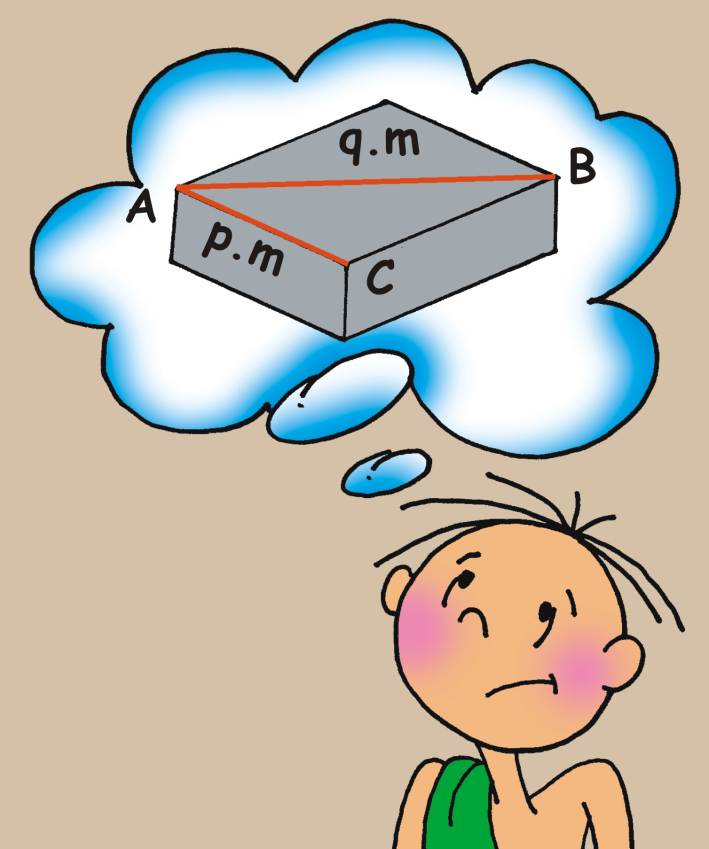
\includegraphics[scale=0.5]{fig-sets/apoloa.png}
\end{center}
\end{wrapfigure}
Equation~\ref{Pytagoras1} shows that $q$ is even;
equation~\ref{peven} proves that $p$ is even too. But this is against our
assumption that $p$ and $q$ are not both even. Therefore, $p$ and $q$ cannot be
integers in equation~\ref{Pytagoras1}, which you can rewrite as
$$\frac{p}{q}=\sqrt{2}$$



The number $\sqrt 2$, that gives the ratio
between the side and the diagonal of any square, is not an element of $\mathbb{Q}$,
or else, $\sqrt 2 \notin  \mathbb{Q}$. It was Hypasus of Metapontum, a Greek philosopher,
who proved this. The Greeks were a people of wise men and women. Nevertheless they
had the strange habit of consulting with an illiterate peasant girl at Delphi,
before doing anything useful. Keeping with this tradition, Hyppasus  asked
the Delphian priestess--- the illiterate girl--- what he should do to please Apollo.
She told him to measure  the side and the diagonal of the god's square
altar using the same meter. By proving
that the problem was impossible, Hypasus discovered a type of number that can not be
written as a fraction. This kind of number is called irrational.

An irrational number
is not a crazy, or a stupid number; it is simply a number that you cannot represent
as {\em ratione} (fraction, in Latin).

The set of all numbers, integer, 
irrational, and rational is called $\mathbb{R}$, or
the set of real numbers. 

Computers are not able to deal
with sets that hold a transfinite number of
elements. Therefore, scheme and
all other programming languages
replace sets with the concept of type.
In scheme, $\mathbb{Z}$ is 
called {\bf integer}, although
the {\bf integer} type does not cover all integers, 
but enough of them to satisfy
your needs. Likewise, a floating point
number belongs to the {\bf number} type, 
which is a subset of $\mathbb{R}$.


If $x\in{\bf Int}$, Lisp programmers\index{Type} say 
that $x$ has 
type\label{type:definition} \index{Type!Int} {\bf integer}. 
They also say that $r$ has 
type {\bf number} if $r\in {\bf Real}$.

In scheme, rational and irrational numbers
are inexact data types. Here are a few functions
that produce inexact results:
\begin{quote}
$\verb|(+ |x_1\;x_2\;\ldots x_n\verb|)|$ -- addition\\
$\verb|(* |x_1\;x_2\;\ldots x_n\verb|)|$ -- multiplication\\
$\verb|(- |x_1\;x_2\;\ldots x_n\verb|)|$ -- subtraction\\
$\verb|(/ |x_1\;x_2\;\ldots x_n\verb|)|$ -- division\\
$\verb|(expt |x\;y\verb|)|$ -- $x^y$\\
$\verb|(sin | x \verb|)|$ -- $\sin(x)$\\
$\verb|(asin | x \verb|)|$ -- $\arcsin(x)$\\
$\verb|(cos | x \verb|)|$ -- $\cos(x)$\\
$\verb|(acos | x \verb|)|$ -- $\arcsin(x)$\\ 
$\verb|(tan | x \verb|)|$ -- $\tan(x)$\\
$\verb|(atan | x \verb|)|$ -- $\arctan(x)$\\
$\verb|(log | x \verb|)|$ -- natural logarithm\\
\end{quote}\index{Predicates!integer?}
Integers are distinguished from inexact numbers
by the \verb|(integer? x)| predicate. Two important
integer functions are \verb|(quotient x y)| and
\verb|(remainder x y)|. The first function
produces the integer division of \verb|x|
by \verb|y|, while the other returns
the remainder of the division. You should remember
having used
these two functions earlier to calculate the Zeller's
congruence.

\section{Data types}
There are other types
besides {\bf integer}, and {\bf number}. 
Here is a  list of primitive types:
\begin{description}
\item[integer ---] Integer numbers between $-2147483648$ and $2147483647$. \index{Predicates!exact?}
The \verb|(exact? x)| function returns \verb|#t| if \verb|x|
is an integer, and \verb|#f| otherwise.
\item[inexact ---] the inexact type represents both
rational and irrational numbers, albeit approximately.
The \verb|(inexact? x)| function returns \verb|#t| for
inexact numbers.\index{Predicates!inexact?}
\item[number ---] A number can be either exact or inexact.
The \verb|(number? x)| function returns \verb|#t| for numbers,
and \verb|#f| for any other type of object.\index{Predicates!number?}
\item[String ---] A quoted\index{String} string \index{Type!String}
of characters: \verb|"3.12"|, \verb|"Hippasus"|, \verb|"pen"|, etc.
The \verb|(string? x)| function answers \verb|#t| 
if \verb|x| is a string, 
and \verb|#f| otherwise.\index{Predicates!string?}
A few important functions that operate on strings are:
\begin{itemize}
\item \verb|(string-length s)| returns the number
of chars of the \verb|s| string.
\item\verb|(substring "Hello, World" 2 5)| operation
returns the \verb| "llo"| substring.
\verb|(substring "Hello, World" 0 4)| returns the
\verb|"Hell"| substring. And so on.
\end{itemize}
\item[Char ---] Chars have the \verb|#\|
  prefix: \index{Type!Char}
\verb|#\A|,
\verb|#\b|, \verb|#\3|, \verb|#\space|,
\verb|#\newline|, etc.
The \verb|(char? x)| function returns \verb|#t|
when \verb|x| is a char.\index{Predicates!char?}
Let \verb|s| be
a string such as \verb|"Hello"|. Then,
\verb|(string-ref "Hello" 0)|
returns the first char of \verb|s|,
\verb|(string-ref "Hello" 1)| returns
the second char, and so on. One can compare
chars with the following functions:
\begin{quote}
\verb|(char=? x #\g)| -- \verb|#t| if \verb|x= #\g|\\
\verb|(char>? x #\g)| -- \verb|#t| if \verb|x| comes
after the \verb|#\g| char.\\
\verb|(char<? x #\g)| -- \verb|#t| if \verb|x| comes
before the \verb|#\g| char.\\
\verb|(char>=? x #\g)| -- \verb|#t| if \verb|x| is
equal to \verb|#\g| or comes after it.\\
\verb|(char<=? x #\g)| -- \verb|#t| if \verb|x| is
equal to \verb|#\g| or comes before it.\\
\end{quote}
\item[Pair ---] One can use a pair data type
both to represent Cartesian pairs and lists.
The \verb|(pair? x)| returns \verb|#t| if
\verb|x| is a pair,\index{Predicates!pair?}
otherwise it returns \verb|#f|.
The \verb|'()| empty list is a very important
object that one can use as the second element
of a pair. The \verb|(null? x)| returns \verb|#t|
when \verb|x| is the \verb|'()| empty list.
\end{description}


\section{Functions}
A function is a relationship between an argument and a unique value.
Let the argument be $x\in B$, where $B$ is a set; then $B$ is called
domain of the function. Let the value be $f(x)\in C$, where $C$ is
also a set; then $C$ is the range of the function.
Functions can be represented by tables, or clauses. Let us examine
each one of these representations in turn.

\subsection*{Tables}
Let us consider a function that associates \verb|#t| ({\em true})
or \verb|#f| ({\em False}) to the
letters of the Roman alphabet. If a letter is a vowel,
then the value will be \verb|#t|; otherwise, 
it will be \verb|#f|. The range of such a function
is \verb|{#t, #f}|, and the domain is
$\{a,b,c,d,e,f,g,h,i,j,k,l,m,n,o,p,q,r,s,t,u,v,w,x,y,z\}$.\\

\verb||\\
{\footnotesize
\begin{tabular}{|p{1.2cm} p{1.2cm} | p{1.2cm} p{1.2cm} |p{1.2cm} p{1.2cm} | p{1.2cm} p{1.2cm} |}
Domain & Range & Domain & Range & Domain & Range & Domain & Range\\
a & \verb|#t| & g &\verb|#f| & m &\verb|#f| & t & \verb|#f| \\
b & \verb|#f| & h &\verb|#f| & n & \verb|#f| & u & \verb|#t| \\
c & \verb|#f| &  i &\verb|#t| &o &\verb|#t| & v & \verb|#f|\\
d &\verb|#f| &  j & \verb|#f| & p & \verb|#f| & w & \verb|#f| \\
e &\verb|#t| & k & \verb|#f| & q & \verb|#f| & x & \verb|#f| \\
f &\verb|#f| &  l &\verb|#f| & r & \verb|#f| & y & \verb|#f| \\
&            &                 &  & s & \verb|#f| & z & \verb|#f|\\
\end{tabular}}

\subsection{Clauses}
From what you have seen in the last section, you certainly notice that it is pretty tough to represent a
function using a table. You must list every case. There are also functions,
like $\sin\;x$, whose domain has an infinite number of values, which makes
it impossible to list all entries. 
Even if you were to try to insert only a finite
subset of the domain into the table, it wouldn't be easy. 
Notwithstanding, in the past,
people used to build tables. In fact, tables were the only way to calculate many
useful functions, like $(\sin\;x)$, 
$(\log\;x)$, $(\cos\;x)$, etc. In 1814 Barlow
published his Tables which give factors, squares, cubes, square roots, reciprocals
and hyperbolic logs of all numbers from 1 to 10000. In 1631 Briggs published
tables of sin functions to 15 places and tan and sec functions to 10 places.
I heard the story of a mathematician who published a table of sinus, and made
a mistake. Troubled by the fact that around a hundred sailors lost their way due to his
mistake, that mathematician committed suicide. This story shows that the use
of tables may be hazardous to your health.

In order to understand how to represent a function with clauses, let us revisit the vowel table.
Using clauses, that table becomes
\begin{quote}\small
\begin{verbatim}
(define (vowel x)
  (cond ( (or (char=? x #\a)(char=? x #\e)(char=? x #\i) 
              (char=? x #\o)(char=? x #\u)) #t)
    (else #f)))
\end{verbatim}
\end{quote}
Expressions like $(\verb|or | p_1\;p_2\ldots p_n)$ has the same 
meaning as $p_1 \vee p_2\ldots \vee p_n$.

Functions have a parameter, also called variable, that represents an element of the domain.
Thus, the vowel function has a parameter \verb|x|, that represents an element of the set
\verb|{'a','b','c','d','e','f',...}|.
Below the name of the function, and its variable, one finds a set of clauses.
Each clause has a condition followed by an expression, that gives the value,
if that clause applies. Consider the first clause. The expression:
\begin{quote}
\begin{verbatim}
(or (char=? #\a)(char=? #\e)(char=? #\i)
    (char=? #\o)(char=? #\u))
\end{verbatim}
\end{quote}
asks the question: {\em Is \verb|x= #\a|,
\verb|x= #\a|, \verb|x= #\a|, \verb|x= #\a| or
\verb|x= #\a|?} If the answear is yes,
the  clause  value is \verb|#t|; in proper functions,
the clause
value is given by the second clause expression. 

Now, let us consider the Fibonacci function,
that has such an important role in the
book ``The Da Vinci Code''.
Here is its table for the first 6 entries:\\
\begin{quote}\label{page:Fibonacci}
\begin{tabular}{p{2cm}p{3cm} | p{2cm}p{3cm}}
0 & 1 & 3 & 3 \\
1 & 1 & 4 & 5  \\
2 & 2 & 5 & 8
\end{tabular}
\end{quote}
Notice that a given functional value is equal
to the sum of the two precedent values,
i.e.,  $f_{n+1}= (+\;f_n\;f_{n-1})$. Assume that $n=5$. 
Then,  $f_6= (+\;f_5\;f_4)$.

Of course, the expression
$f_{n+1}= (+\;f_n\;f_{n-1})$
is true only for $n>0$,
since there are not two precedent
values for $n+1=0$, or $n+1=1$. 
The below programa shows how  you can state that a rule
is valid only under certain conditions.\\

\begin{fmpage}{0.9\linewidth}
\begin{verbatim}
(define (fib n fn fn-1)
(cond ((< n 2) fn)
    (else  (fib (- n 1) (+ fn fn-1) fn)) ))
\end{verbatim}
\end{fmpage}

\begin{fmpage}{0.9\linewidth}
\begin{verbatim}
1:=> (load "fibonacci.scm")
fibonacci.scm
1:=> (fib 5 1 1)
8
\end{verbatim}
\end{fmpage}


\paragraph{Predicates.} A predicate
is a function that gives
true and false for output. In Scheme,
the only false value is \verb|#f|, but
any value that is different from \verb|#f|
is considered true. A predicate can be used to discover
whether a property is true for a given value.
For instance, a sequence of elements
such as \verb|'(S P Q R)| is called
list. There is also an empty list,
that has no elements at all, and
is represented by \verb|'()|. Let
\verb|xs| be a list. Then, the predicate
\verb|(null? xs)| returns \verb|#t|
if \verb|xs| is the empty list.

There are predicates designed for
performing comparisons. For instance,
\verb|(> m 2)| returns \verb|#t| for
\verb|m| greater than 2, and \verb|#f|
otherwise. Here is a more or less complete
list of comparison predicates:
\begin{itemize}
\item\verb|(> m n)| -- \verb|#t| for
\verb|m| greater than \verb|n|.
\item\verb|(< m n)| -- \verb|#t| for
\verb|m| less than \verb|n|.
\item\verb|(>= m n)| -- \verb|#t| for
\verb|m| greater or equal to \verb|n|.
\item\verb|(<= m n)| -- \verb|#t| for
\verb|m| less or equal to \verb|n|.
\item\verb|(= m n)| -- \verb|#t| if
\verb|m| is a number equal to \verb|n|.
\end{itemize}
The inputs \verb|m| and \verb|n| must
be both numbers, if you want
the above predicates to work.


A string is a sequence of characters
represented between double quotation
marks. For instance, \verb|"Sunday"|
is a string. Below, there is a short
list of string predicates.
\begin{itemize}
\item\verb|(string=? s z)| -- \verb|#t|
if \verb|s| and \verb|z| are equal.
\item\verb|(string>? s z)| -- \verb|#t|
if \verb|s|  comes
after \verb|z| in the alphabetical order.
\item\verb|(string<? s z)| -- \verb|#t|
if \verb|s| comes before \verb|z|
in the alphabetical order.
\item\verb|(string<=? s z)| -- \verb|#t| if
\verb|s| precedes or is equal to \verb|z|.
\item\verb|(string>=? s z)| -- \verb|#t| if
\verb|s| follows or is equal to \verb|z|.
\end{itemize}

The prefix \verb|#\| identifies isolated
characters. Let us assume the following
definition:
\begin{quote}
\begin{verbatim}
(define s "Nia Vardalos")
\end{verbatim}
\end{quote}
Then, the characters
\verb|#\N| \verb|#\i| 
\verb|#\a| and \verb|#\space|
were retrieved from
\verb|s| by the
expressions \verb|(string-ref s 0)|,
\verb|(string-ref s 1)|,
\verb|(string-ref s 2)| and
\verb|(string-ref s 3)|,
\verb|| respectively.

The blank space character,  control
characters, non-graphic characteres
and all other non-printable characters
can be represented by
identifiers, such as \verb|#\space|,
\verb|#\tab| and \verb|#\newline|.

Character have their own set of
predicates, as one should expect.
\begin{itemize}
\item\verb|(char=? #\A #\a)| -- is \verb|#f|
since \verb|#\A| and \verb|#\a| are not equal.
\item\verb|(char>? #\z #\a)| -- is \verb|#t|
since \verb|#\z|  comes
after \verb|#\a| in the alphabetical order.
\item\verb|(char<? #\a #\z)| -- is \verb|#t|
since \verb|#\a| comes before \verb|#\z|
in the alphabetical order.
\item\verb|(char<=? #\a #\c)| -- is \verb|#t| since
the order of \verb|#\a| is less or equal to
the order of \verb|#\c|.
\item\verb|(char>=? #\a #\c)| -- \verb|#f| since
the order of \verb|#\a| greater or equal to the
order of \verb|#\c|.
\end{itemize}

Besides predicates, Scheme uses special forms
to make decisions. The $(\textrm{and}\; p_1\;
p_2\ldots p_n)$ form
evaluates the sequence $p_1$, $p_2$\ldots $p_n$
until it reaches $p_n$ or one of the previous
$p_i$ returns \verb|#f|. In fewer words,
the and-form stops at the first
$p_i$ that returns \verb|#f| and, if no
argument is false, it stops at $p_n$.
The form returns the value of the last
$p_i$ that it evaluates. The and-form
returns a value different from \verb|#f|
if and only if all $p_i$ predicates produce
values different from \verb|#f| (false).

Like the and-form, the or-form also stops
as soon as it can. In the case of the or-form,
this means returning true as soon as any
of the arguments is true. Remember that
true is anything different from \verb|#f|.
The  $(\textrm{or}\; p_1\;
p_2\ldots p_n)$ form returns the value
of the first true $p_i$ predicate.

The \verb|(not P)| form returns \verb|#t|
if \verb|P| produces \verb|#f|, and
evaluates to \verb|#f| if \verb|P| is true,
i.e., anything different from \verb|#f|.

With the and, or and not forms, Nia can
combine primitive functions to define
many interesting predicates. For instance,
the predicate \verb|(digit? d)| determines
wether \verb|d| is a digit.
\begin{quote}
\begin{verbatim}
(define (digit? d)
(and (char>=? d #\0)
     (char<=? d #\9)))
\end{verbatim}
\end{quote}
The predicate \verb|deep-winter?| checks if
\verb|m| is 1 or 2:
\begin{quote}
\begin{verbatim}
(define (deep-winter? m)
   (or (= m 1) (= m 2)))
\end{verbatim}
\end{quote}


\section{The cond-form}\label{page:cond-form}
Now that Nia knows how to find
an integer between 0 and 6 for the 
day of the week, she needs a function
that produces the corresponding name.


\begin{figure}[!h]
\begin{fmpage}{\linewidth}
\begin{verbatim}
(define (week-day n)
   (cond [ (= n 0) 'Sunday]
      [ (= n 1) 'Monday]
      [ (= n 2) 'Tuesday]
      [ (= n 3) 'Wednesday]
      [ (= n 4) 'Thursday]
      [ (= n 5) 'Friday]
      [ else 'Saturday]))

(define (zeller y m day)
  (let* [ (roman-month (if (< m 3) (+ m 10) (- m 2)))
          (roman-year (if (< m 3) (- y 1) y))
          (century (quotient roman-year 100))
          (decade (remainder roman-year 100)) ]
     (week-day (remainder (+ day decade
                   (quotient (- (* 13 roman-month) 1) 5)
                   (quotient decade 4)
                   (quotient century 4)
                   (* century -2)) 7)) ))
\end{verbatim}
\end{fmpage}

\begin{fmpage}{\linewidth}
\begin{verbatim}
1:=> (load "zellerCond.scm")
zellerCond.scm
1:=> (zeller 2018 8 31)
Friday
\end{verbatim}
\end{fmpage}
\caption{Day of the week}
\label{fig:day-of-the-week}
\end{figure}

\index{Conditional execution!cond}
\index{cond!clauses}
The cond-form controls conditional
execution, based on a set of clauses.
Each clause has a condition followed by
a sequence of actions.  Lisp starts with the
top clause, and proceeds in decending order.
It executes the first clause whose 
condition produces a value different from \verb|#f|.
For instance, the first clause condition is
the \verb|(= n 0)| predicate.
If the predicate \verb|(= n 0)| 
returns \verb|#t| for the Sunday index,
the function \verb|week-day| returns \verb|'Sunday|.
If \verb|n= 1|, the second condition holds,
and the function produces the symbol \verb|'Monday|.
And so on.


\section{Lists}
In Lisp, there is a data structure called list,
that uses parentheses to represent nested
sequences of objects. One can use lists to
represent structured data.
For instance, in the snippet below,
\verb|xor-structure| shows
the structure of a combinatorial circuit
through nested lists.

\begin{verbatim}
(define *x* 42)

(define xor
  (lambda(A B)
    (or (and A (not B))
        (and (not A) B)) ))

(define xor-structure
  '(or (and A  
            (not B))
       (and (not A) 
            B)))
\end{verbatim}

Although Nia does not know what a combinatorial 
circuit is, she noticed that the structure
defined as \verb|xor-structure| is prefixed by a
single quotation mark, that in Lisp parlance is
known as quote. Since Scheme uses the
same notation for programs and structured
data, the computer needs a tag to set
data apart from code. Therefore, 
quote was chosen to indicate that
an object is a list, not a procedure that
needs to be executed by the computer.

The \verb|define| form creates global
variables. In the above source code,
the variable \verb|*x*| is an id for the
number 42,
while \verb|xor| is the id for a program
that calculates the output of a two
input exclusive or gate. Of course, Nia
could define the \verb|xor| gate as shown below:
\begin{verbatim}
(define *x* 42)

(define (xor A B)
  (or (and A (not B))
      (and (not A) B)) )

(define xor-structure
  '(or (and A 
            (not B))
       (and (not A) 
            B)))
\end{verbatim}

From the examples, Nia discovered that there
are two ways of defining the \verb|xor| gate
as a combination of \verb|A| input, \verb|B| input,
\verb|and| gate, \verb|or| gate
and \verb|not| gate. In the first and
most popular style, one uses the
\verb|(xor A B)| format that is a mirror of
the gate application. The advantage of
this method is that it spares one
nesting level, and shows clearly how to use
the definition. 

In the second style of defining functions and
gates, the id of the abstraction 
appears immediately after the \verb|define|
keyword. The  arguments and the body of
the definition are introduced by a lambda form:
\label{page:lambda1}\index{lambda}

\begin{verbatim}
(define xor
  (lambda(A B)
    (or (and A (not B))
        (and (not A) B)) ))
\end{verbatim}

This second style is quite remarkable because
the abstraction that defines the operation
is treated exactly like any other
data type existent in the language.
In fact, there is no formal difference
between the definition of \verb|*x*|
as an integer constant, and \verb|xor|
as a functional abstraction.

\begin{figure}[!h]
\begin{fmpage}{0.8\linewidth}
\begin{verbatim}
; File: lists.scm

(define xor-structure
  '(or (and A (not B))
       (and (not A) B)))
\end{verbatim}
\end{fmpage}

\begin{fmpage}{0.8\linewidth}
\begin{verbatim}
1:=> (load "lists.scm")
lists.scm
1:=> (car xor-structure)
or
1:=> (cdr xor-structure)
((and A (not B)) (and (not A) B))
1:=> (car (cdr xor-structure))
(and A (not B))
1:=> (car (cdr (car (cdr xor-structure))))
A
1:=> (car (cdr (cdr (car (cdr xor-structure)))))
(not B)
\end{verbatim}
\end{fmpage}

\begin{fmpage}{0.8\linewidth}
\verb||
\end{fmpage}
\caption{List selectors}
\label{fig:selectors}
\end{figure}


Although Scheme represents programs and
data in the same way, it does not use
the same methods to deal with source
code and lists. In the case of source
code, the compiler translates it into
a virtual machine language that the
computer can easily and efficiently
process.

Data structures, such as lists, have
an internal representation with parts. 
In particular, a list is implemented
as a chain of pairs 
(vide page~\pageref{page:cartesian-pair}),
each pair containing
a pointer to a list element,
and another pointer to the next pair. 
Let us assume that
\verb|xs| points to the list
\verb|'(S P Q R)|.
This list corresponds to the following
chain of pairs:
\begin{quote}
\begin{verbatim}
[*|*]--->[*|*]--->[*|*]--->[*|*]--->()
|        |        |        |        
S        P        Q        R       
\end{verbatim}
\end{quote}
The first pair has a pointer to \verb|S|,
and another pointer to the second pair.
The second pair contains pointers to 
\verb|P| and to the third pair. 
The third pair points to \verb|Q| and
to the fourth pair. Finally, the fourth
pair points to \verb|R| and to 
the \verb|()| empty list.

\begin{quote}
\begin{verbatim}
[*|*]---> next pair
|        
S      
\end{verbatim}
\end{quote}
The operation \verb|(car xs)| produces
the first pointer of the \verb|xs| 
chain of pairs. In the case of
the \verb|'(S P Q R)| list, \verb|(car xs)|
returns \verb|S|. On the other hand,
\verb|(cdr xs)| yields the pair
after the one pointed out by \verb|xs|,
i.e., \verb|'(P Q R)|. A sequence
of \verb|cdr| applications permits the user to
go through the pairs of a list. \\

\begin{fmpage}{0.8\linewidth}
\begin{verbatim}
(define spqr
   '(S P Q R))
\end{verbatim}
\end{fmpage}

\begin{fmpage}{0.8\linewidth}
\begin{verbatim}
1:=> (load "spqr.scm")
spqr
1:=> spqr
(S P Q R)
1:=> (cdr spqr)
(P Q R)
1:=> (cdr (cdr spqr))
(Q R)
1:=> (cdr (cdr (cdr spqr)))
(R)
\end{verbatim}
\end{fmpage}

\begin{fmpage}{0.8\linewidth}
\verb||
\end{fmpage}


If all one needs is to represent
sequences, then contiguous memory
elements could be more
practical than pairs. However, as one
can see in figure~\ref{fig:selectors},
a list element can be a nested sublist.
In this case, 
the \verb|car| part of a pair can point down to
a sublist branch. The diagram below shows
that one can reach any part of a nested
list following a chain of \verb|car| and \verb|cdr|.
In such a chain, the \verb|cdr| operation
advances one pair along the list, and
the \verb|car| operation goes down into a sublist.
The \verb|cdr| operation is equivalent to a
right $\rightarrow$  arrow, while the \verb|car|
operation is acts like a down $\downarrow$ arrow.
\begin{quote}
\verb"     "$\rightarrow$\verb"       "$\rightarrow$\\
\verb"[*|*]cdr-[*|*]cdr---[*|*]--()"\\
\verb" |        |         car"$\downarrow$\\
\verb" |        |          |  " $\rightarrow$\\
\verb" |        |         [*|*]cdr-[*|*]---[*|*]---()"\\
\verb" |        |          |       car"$\downarrow$\verb"     |"\\
\verb" |        |          |        |       |"\\
\verb" |        |          |        |       B"\\
\verb" |        |          |        |  "\\
\verb" |        |         and      [*|*]---[*|*]---()"\\
\verb" |        |                   |       |"\\
\verb" |        |                   |       |"\\
\verb" |        |                  not      A"\\
\verb" |        |"\\
\verb" or      [*|*]---[*|*]---[*|*]---()"\\          
\verb"          |       |       |"\\                     
\verb"         and      A      [*|*]---[*|*]---()"\\  
\verb"                          |       |"\\                     
\verb"                         not      B"                    
\end{quote}
The above example shows the chains and subchains of
pairs that one uses to represent the logic
circuit below:
\begin{quote}
\begin{verbatim}
(define xs
'(or 
     (and  A  
           (not B))
                    (and (not A)
                         B)))
\end{verbatim}
\end{quote}

Let us assume that Nia wants to retrieve the
\verb|(NOT A)| part of the circuit. Considering
that each right $\rightarrow$ arrow is equivalent
to a \verb|cdr| operation, and each down $\downarrow$
arrow can be interpreted as a \verb|car| operation,
she must perform \verb|(car (cdr (car (cdr (cdr xs)) )))|
to reach the goal.


\section{Processing text from the editor}
Let us learn how to retrieve a selection such as
\verb|"(2016 8 31)"| from emacs,
transform it into the \verb|'(2016 8 31)|
list, and calculate the corresponding
day of the week.

To select the string, press \verb|C-Spc|
at the first character, and
move the cursor onto the last character.

The problem is that the clipboard
contains a string like \verb|"(2016 8 31)"|, and
the \verb|zeller| function defined in needs a list.
Therefore, Nia needs a procedure to
read a list from a string of characters.

All languages open ports for reading things
from files. Lisp is no exception, but for
the fact that one can open objects like
strings, and read complex objects such
as a whole list. These powerful features
can be seen in the above definition.
The \verb|let*| was necessary in the 
definition of \verb|read-string| because
Nia needs the result of \verb|(read port)|,
and cannot close the port before finishing
the reading. The solution for this problem
is to execute \verb|(read port)|, 
the \verb|(close-input-port port)|, and
finally return the produce of \verb|(read port)|,
which is stored in the variable \verb|res|.

To solve the proposed problem, you will need to load
the \verb|readfromstring| file and also the definition
of Zeller's congluence, given on
page~\pageref{fig:day-of-the-week}.

\begin{verbatim}
;; File readfromstring.scm

(define (rdstr str)
  (let* [ (port (open-input-string str))
          (res (read port))]
      (close-input-port port) res) )

#|
1:=> (load "readfromstring.scm")
readfromstring.scm
1:=> (load "zellerCond.scm")
zellerCond.scm
1:=> (zeller 2016 8 31)
Wednesday
1:=> (apply zeller (rdstr "(2016 8 31)"))
Wednesday
|#
\end{verbatim}

As you can see above, you can place text between
\verb/#|/ and \verb/|#/ to mark it as comment.
From now on, this book will show how to use a
program by placing an example between comment marks.

\section{The list constructor}\index{List!cons}
Since the \verb|car| and \verb|cdr| operations
select the two parts of a pair, they are called
{\em selectors}.
Besides the two selectors, lists have a
constructor: The operation \verb|(cons x xs)| builds a pair
whose first element is \verb|x|, and the 
remaining elements are grouped in \verb|xs|.

\begin{quote}
\verb|(cons 'and '(A B))|\keys{Enter}\\
(and A B)
\end{quote}

One has learned previously that lists must be
prefixed by the special quote operator,
in order to differentiate them from programs.
To make a long story short, quote  prevents
the evaluation of a list or symbol.

When you first heard about pairs on
page~\pageref{page:cartesian-pair},
it was stated that the first element
of a pair is separated from the 
second by a dot. However, the dot
can be omitted if the second element
is itself a cartesian pair or
the empty list. Then,
the  much neater 
\verb|'(3 4)| list syntax is equivalent 
to the dotted Cartesian \verb|'(3 . (4 . ()))| pair.

A backquote, not to be confused with quote, also prevents
evaluation, but the backquote transforms the list 
into a template.\index{List!backquote}
When there appears a comma in the 
template, Lisp evaluates the expression following
the comma\index{List!comma}
and replaces it with the result. 
If a comma is combined with \verb|@| to produce
the \verb|,@| at-sign,\index{List!at-sign}
then the expression following the at-sign 
is evaluated to create a list. This list is
spliced into place in the template. 
Templates are specially useful for creating
macros, as you will learn below.

\index{Macros!define-syntax}
\begin{verbatim}
(define-syntax while-do 
  (syntax-rules ()
    [ (kwd condition the-return  bdy ...)
      (do () ((not condition) the-return) bdy ...)]))

(define (reverse-iota m)
  (let [(s '()) (i 0)]
    (while-do (< i m) s
	    (set! s (cons i s))
	    (set! i (+ i 1)) )))
#|
1:=> (load "whiledo.scm")
whiledo.scm
1:=> (reverse-iota 5)
(4 3 2 1 0)
|#
\end{verbatim}


Macros are programs that brings a more convenient
notation to a standard Lisp form. The syntax of Lisp,
that unifies data and programs, makes it possible to
create powerful macros that implement Domain Specific
Languages (DSLs), speed up coding or create new software
paradigms. In fact, the macro system is one of the
two features that places Lisp asunder from other
languages, the other being its Mathematical Foundations.

In the above macro definition, the \verb|syntax-rules|
have the form
\begin{quote}
\verb|(syntax-rules (keyword ...) clause ...)|
\end{quote}
Clauses have the form \verb|(pattern template)|,
where each pattern shows one possible syntax.
The templates specify how the pattern should
be expanded to create a valid Lisp expression.
A pattern may contain keywords, variables and
ellipses. An ellipsis \verb|...| indicates that
the previous expression can be followed by other
expressions with the same shape. The syntax of
Lisp requires that a blank space is inserted before
and after an ellipsis. A keywords is
an identifier that only matches itself.


\chapter{Recursion}\label{chapter:Recursion}
\index{Recursion}
The mathematician Peano invented a very interesting axiomatic theory for
natural numbers. I cannot remember the details, but the idea was
something live the following:
\begin{enumerate}\index{Recursion!Peano's axioms}
\item Zero is a natural number.
\item Every natural number has a successor: The successor of 0 is 1, the
successor of 1 is 2, the successor of 2 is 3, and so on.
\item If a property is true for zero and, after assuming that it is true for n,
you prove that it is true for n+1, then it is true for any natural number.
\end{enumerate}
Did you get the idea? For this very idea can be applied to many other
situations. When they asked Myamoto Musashi, the famous Japanese
Zen assassin, how he managed to kill a twelve year old boy protected by his
mother's 37 samurais, he answered:
\begin{quote} \em
I defeated one of them, then I defeated
the remaining 36. To defeat 36, I defeated one of them, then I defeated
the remaining 35. To defeat 35, I defeated one of them, then I defeated the
remaining 34\ldots \\
\ldots~~~~~~~\ldots~~~~~~~\ldots\\
To defeat 2, I defeated one of them, then I defeated the other.
\end{quote}
A close look will show that 
the function \index{Recursion!Append!Definition}
\verb|App| of Listing~\ref{rec/app} acts like
Musashi. The first
clause of \verb|(App xs s)| states that
appending a \verb|(null? xs)| list to
\verb|s| produces \verb|s|. The second 
clause of \verb|(App xs s)|  states: To
append a \verb|xs| list to an \verb|s| list,
rewrite the calling 
\verb|(App xs s)| expression as
\begin{quote}
  \verb|(cons (car x) (App (cdr xs) s))|
\end{quote}
Let us pick a more concrete instance of the problem.
The calling pattern \verb|(App '(1 2 3) '(4 5))|
 matches to
\verb|(App xs s)|
with \verb|xs= '(1 2 3)| and \verb|s= '(4 5)|.
Since \verb|(null? xs)| is false, the second
clause rewrites the calling pattern as:
\begin{quote}
\verb|(cons (car xs) (App (cdr xs) s))|
\end{quote}
which the inference engine reduces to 
\begin{equation}
\verb|(cons 1 (App '(2 3) '(4 5)))|
\label{app:1}
\end{equation}
The \verb|(App '(2 3) '(4 5))| subpattern
matches once again with \verb|(App xs s)|,
this time making \verb|xs= '(2 3)|
and \verb|s= '(4 5)|. Since \verb|(null? xs)|
is false, the second clause holds, and the
\verb|(App '(2 3) '(4 5))| is rewritten as
\begin{quote}
\verb|(cons 2 (App '(3) '(4 5)))|.
\end{quote}
Therefore, equation~\ref{app:1} becomes:
\begin{equation}
\verb|(cons 1 (cons 2 (App '(3) '(4 5))))|
\label{app:2}
\end{equation}

The calling pattern \verb|(App '(3) '(4 5))|
matches to \verb|(App xs s)| with
\verb|xs= '(3)| and \verb|s= '(4 5)|.
For the last time, the second clause is
chosen, and expression~\ref{app:2} becomes:
\begin{equation}
\verb|(cons 1 (cons 2 (cons 3 (App '() '(4 5)))))|
\label{app:3}
\end{equation}
The pattern \verb|(App '() '(4 5))| matches
to \verb|(App xs s)| with \verb|xs= '()|
and \verb|s= '(4 5)|. This 
time, \verb|(null? xs)| is true,
and the calling pattern reduces to \verb|s|,
which is equal to \verb|'(4 5)|, and
expression~\ref{app:3} can be rewritten as:
\begin{quote}
\verb|(cons 1 (cons 2 (cons 3  '(4 5))))= '(1 2 3 4 5)|
\end{quote}


\begin{figure}[!b]
\begin{fmpage}{0.8\linewidth}
\begin{verbatim}
(define (App xs s)
  (cond [ (null? xs) s]
    [else (cons (car xs) (App (cdr xs) s)) ]))
\end{verbatim}
\end{fmpage}

\begin{fmpage}{0.8\linewidth}
\begin{verbatim}
1:=> (App '(1 2 3) '(4 5))
(1 2 3 4 5)
\end{verbatim}
\end{fmpage}
\caption{Append}
\label{rec/app}
\end{figure}


\section{Classifying rewrite rules}\index{Recursion!Classifying rules}
Typically a recursive definition has two kinds of clauses:
\begin{enumerate}
\item Trivial cases, which can be \index{Recursion!Trivial case} 
resolved using primitive operations.
\item General cases, which can be \index{Recursion!General case} 
broken down into simpler cases.
\end{enumerate}
Let us classify the two clauses of \verb|(App xs s)|:\\

\verb||\\
\begin{tabular}{p{5cm}p{7cm}}
\verb|[(null? xs) s]| & The first clause is certainly trivial\\
\\
\verb|[else |

\verb|  (cons (car xs)|

\verb|    (App (cdr xs) s))]|
& The second equation can be
broken down into simpler
operations: Appending two
lists with one element
removed from the first,
and then inserting the element
left out into the result.\\
\end{tabular}


\section{Quick Sort}
Although Hoare's Quick Sort algorithm is
of little practical use in these days of BTree everywhere, it gives a good illustration
of recursion. The problem that Hoare solved consists of sorting a list.

The \verb|(smaller xs p)| function returns
all elements of \verb|s| that are smaller
than the \verb|p| pivot. 
The \verb|(greater xs p)| produces the
list of the \verb|s| elements that are
greater or equal to \verb|p|. Therefore the
\verb|(quick xs)| function partitions 
\verb|xs| into three lists, then sorts
and appends these lists:
\begin{itemize}
\item \verb|(smaller (cdr s) (car s))|--
numbers smaller than \verb|(car s)|
\item \verb|(list (car s))| 
\item \verb|(greater (cdr s) (car s))|--
numbers greater or equal to \verb|(car s)|.
\end{itemize}
If you sort, then concatenate these three lists,
you will end up sorting the original list.
A concrete case will make this fact clear.
Let \verb|s| be the list \verb|'(4 3 1 5 2 8 7)|.
The expression
\verb|(quick (smaller (cdr s) (car s)))|
returns \verb|'(1 2 3)|.
The expression
\verb|(quick (greater (cdr s) (car s)))|
generates \verb|'(5 7 8)|. Finally, 
the 
\verb|(append '(1 2 3) '(4) '(5 7 8))|
application
returns \verb|'(1 2 3 4 5 7 8)|.

In the quicksort algorithm,
there are two trivial cases,
the empty \verb|'()| list
and lists with a single element,
either of which
do not require sorting.

Lists with two or more elements
are sorted by breaking them into
smaller sublists. Since they are
closer to the trivial cases,
one can assume that the smaller sublists
are easier to sort. Figure~\ref{quicksort} shows
a complete implementation of the quicksort algorithm
for a list of numbers.


\begin{figure}[!h]
\begin{verbatim}
;; File: quicksort.scm

(define (smaller xs p)
  (cond [ (null? xs) xs]
     [ (< (car xs) p)
       (cons (car xs)
            (smaller (cdr xs) p))]
     [else (smaller (cdr xs) p)] ))

(define (greater xs p)
  (cond [ (null? xs) xs]
        [ (>= (car xs) p)
          (cons (car xs)
            (greater (cdr xs) p))]
        [else (greater (cdr xs) p)] )) 

(define (quick s)
  (cond [ (null? s) s]
        [ (null? (cdr s)) s]
        [else (append 
                 (quick (smaller (cdr s) (car s)))
                    (list (car s))
                 (quick (greater (cdr s)
                                  (car s))) )] ))

#|
1:=> (load "quick.scm")
quick.scm
1:=> (quick '(8 4 6 3 9 3))
(3 3 4 6 8 9)
|#
\end{verbatim}

\caption{The quicksort algorithm}
\label{quicksort}
\end{figure}

\section{Named-let}

The Fibonacci function on
page~\pageref{page:Fibonacci} has the
undesirable characteristic of
requiring two auxiliary arguments.
Nia cannot forget to initialize
these dummy arguments, otherwise
she will get an error message,
instead of a result. 
The named-let\index{Named-let}\index{Loop!named-let}
permits the creation of functions
with initialized arguments, avoiding
anomolous definitions 
that require manual initialization.

\begin{figure}[!h]
\begin{verbatim}
(define (fibo i)
  (let fn+1 [ (n i) (fn 1) (fn-1 1) ]
    (if (< n 2) fn
        (fn+1 (- n 1) (+ fn fn-1) fn)) ))

;; 1:=> (load "Fibonacci.scm")
;; Fibonacci.scm
;; 1:=> (fibo 5)
;; 8
\end{verbatim}

\caption{One argument Fibonacci function}
\label{oneargfib}
\end{figure}

The named-let binding is used mainly
to loop. In this sense, it is not
different from looping facilities
that one can find in languages like C
or Python. However, the named-let
binding has an important advantage
over other loop facilities: One can
give a meaningful 
name\index{Named-let!meaningful name for loop}
to scheme loops.
For instance, since the loop of
figure~\ref{oneargfib} is used 
to calculate the \verb|fn+1| iteration,
Nia put the \verb|fn+1| tag on it.

On page~\pageref{sec:average}, you learned how to
calculate the average of a list of numbers. Below,
you can see another method of performing the
same task, this time using a named let.

\begin{verbatim}
(define (avg xs)
   (let nxt [(s xs) (acc 0) (n 0)]
     (cond [ (and (null? s) (= n 0)) 0]
         [ (null? s) (/ acc n) ]
         [else (nxt (cdr s) (+ (car s) acc)
                  (+ n 1.0))] )))

;; 1:=> (load "average.scm")
;; average.scm
;; 1:=> (avg '(3 4 5 6))
;; 4.5
\end{verbatim}

\section{Reading data from files}\index{File}

Figure \ref{rdFile} reads and prints a file line by line.
However, before printing a string, \verb|(port->lines p)|
prefixes it with a commented line number. The program should
not print commented lines and empty lines.

\begin{figure}[!h]
\begin{verbatim}
(define (port->lines p)
   (let next-line ( (i 1) (x (read-line p)) )
     (cond [ (eof-object? x) #t]
           [ (< (string-length x) 1)]
           [ (char=? (string-ref x 0) #\;)]
           [else (display "#| ")
              (display (number->string i))
              (cond [ (< i 10)  (display "  |# ")]
                    [else  (display " |# ")])
              (display x) (newline)
              (next-line (+ i 1) (read-line p))] ))) 

(define (rdLines filename)
   (call-with-input-file filename port->lines))

;; 1:=> (load "prtFile.scm")
;; prtFile.scm
;; 1:=> (rdLines "average.scm")
;; #| 1  |# (define (avg xs)
;; #| 2  |#    (let nxt [(s xs) (acc 0) (n 0)]
;; #| 3  |#      (cond [ (and (null? s) (= n 0)) 0]
;; #| 4  |#          [ (null? s) (/ acc n) ]
;; #| 5  |#          [else (nxt (cdr s) (+ (car s) acc)
;; #| 6  |#                   (+ n 1.0))] )))
\end{verbatim}

\caption{Lines from file}
\label{rdFile}
\end{figure}

Lisp has a cleverly designed input system.
The \index{call-with-input-file} \index{Input from file}
\verb|call-with-input-file| \label{page:call-with-input-file}
procedure has two arguments. The first
argument is the file name. 
The second argument is
a single parameter function such
as \verb|port->lines|. In the example
of figure~\ref{rdFile}, Lisp 
opens a file, and pass the file descriptor
to the \verb|port->lines| procedure.

The definition of \verb|(port->lines p)| assigns
a line that it reads  from port \verb|p| to the
variable \verb|x|. Then \verb|x| is printed, and
\verb|loop| proceeds to read the next line. The
iteration stops when  end of file is reached.


\section{Writing data to files}
Let us assume that Nia needs 
a Scheme program that translates
markdown to html. She wants to
use the program to publish poems
in the internet. Here an example
of markdown:
\begin{quote}
\begin{verbatim}
# To Helen
## By Edgard Alan Poe

Helen, thy beauty is to me
Like those Necéan barks of yore,
That gently, o'er a perfumed sea,
The weary, way-worn wanderer bore
To his own native shore.

On desperate seas long wont to roam,
Thy hyacinth hair, thy classic face,
Thy Naiad airs have brought me home
To the glory that was Greece,
And the grandeur that was Rome.

Lo! in yon brilliant window-niche 
How statue-like I see thee stand, 
The agate lamp within thy hand! 
Ah, Psyche, from the regions which 
Are Holy-Land! 
\end{verbatim}
\end{quote}

The program of listing~\ref{wrtFile}
reads a markdown file line by line.
If the line starts with the \verb|##| prefix,
it will be wrapped in the \verb|<h2>...</h2>|
html tag. If its first char is the \verb|#|
prefix, but the second char is different
from \verb|#|, it will be wrapped in
the \verb|<h1>...</h1>| html tag.

The simplified version of the html
generator of listing~\ref{wrtFile} treats
only titles, line breaks and paragraphs.
However, the interested reader will
be able to add other html elements.

You have already learned how the
procedure \verb|call-with-input-file| works.
If you don't remember, take a look at
page~\pageref{page:call-with-input-file}.

The procedure\index{call-with-output-file}
\verb|call-with-output-file|\index{Output to file}
can be\index{Output to file!call-with-output-file}
applied to a file name and a function
with an output port as argument. One could
define the output port function, but
usually people use a lambda abstraction
to perform the magic. Read again the
explanation about the lambda abstraction
on pages~\pageref{page:lambda1}. File
input/output
must be mastered to perfection.

\begin{figure}[!h]
\begin{verbatim}
(define get-line read-line)

(define (tag i <h> x </h> )
   (let [ (Len (string-length x))]
      (string-append <h>
          (substring x i (- Len 1)) </h> "\n")))

(define (subtitle? x)
  (and (> (string-length x) 4)
       (char=? (string-ref x 0) #\#)
       (char=? (string-ref x 1) #\#)))

(define (title? x)
   (and (> (string-length x) 3)
        (char=? (string-ref x 0) #\#)))

(define (convert in out)
  (let loop ( (x (get-line in)) )
     (cond [ (eof-object? x) #t]
        [ (subtitle? x)
          (display (tag 2 "<h2>" x "</h2>") out)
          (loop (get-line in))]
        [ (title? x)
          (display (tag 1 "<h1>" x "</h1>") out)
	  (loop (get-line in))]
        [ (> (string-length x) 1)
          (display x out)
          (display "<br/>\n" out)
          (loop (get-line in))]
        [ else (display "<p/>\n" out)
	    (loop (get-line in))] )))

(define (copyFile inFile outFile)
   (call-with-output-file outFile
      (lambda(out) (call-with-input-file inFile
         (lambda(in) (convert in out))) )))

;; 1:=> (load "prtFile.scm")
;; prtFile.scm
;; 1:=> (load "tohtml.scm")
;; tohtml.scm
;; 1:=> (copyFile "helen.md" "helen.html")
\end{verbatim}

\caption{Writing data to a file}
\label{wrtFile}
\end{figure}



\chapter{Cloud computing}\label{cloud-computing}
A compiler is a program that reads
source code into a language that
human beings can handle easily
and translates the aforementioned
code to an object language that
computers can interpret.
For instance, Nia writes source code
in Low Level Lisp (LLL). The \verb|wasCm| compiler
translates it into WebAssembly Text, or {\em wat}
for short. Then the \verb|wat2wasm| compiler
translates wat code into instructions that the
computer can carry out efficiently.

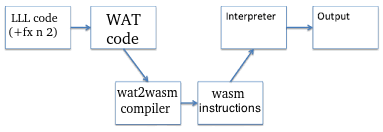
\includegraphics[scale=0.8]{figs/source.png}


The problem is that the \verb|wat2wasm|
compiler installed on
Nia's machine deals with a language
called {\em wat}, while Nia 
works with LLL. Nia can work in a
language different from the compiler
only because the \verb|wasCm| preprocessor
provides a bridge between LLL and the
wat2wasm compiler.


In this chapter, you will learn how
to write a web application in pure
scheme. Thus, you can leap frog
the translation from LLL to {\em wat}.
But firstly,
let us learn what cloud computing is.

Cloud computing is an Internet based
computer that provides shared
processing  on demand for those people
connected to a service provider.
When a  company adheres to cloud computing,
it avoids infrastructure costs,
such as purchasing servers, and keeping
them in working order.

The \verb|https://www.cloudorado.com|
site shows that provider fees
can be pretty steep.
However, one can hire a normal
hosting service and use it for
creating pages that are able to
run quite interesting applications.

When you hire a hosting service,
you will receive a user name and
will be requested to
buy a domain name. Let us
assume that Nia owns the
\verb|medicina.tips| domain,
where {\sc medicina} means
health care in Latin. The domain
may be any sequence of chars,
but it is a good idea to choose
names that raise interest in
Web users. Since doctors usually
know some Latin, if one wants to offer
expert medical consultancy, \verb|medicina.tips|
is a good name.
Now that Nia has a user name and a
domain, she must install scheme servelets
in her cloud machine. Here is how
she enters the shell:
\begin{quote}
\begin{verbatim}
~$ ssh -p2222 nia@medicina.tips
nia@medicina.tips's password: ***
\end{verbatim}
\end{quote}
The 2222 port is used in the secure shell protocol
that connects Nia to the cloud computer.
She needs a password to complete the connection.
\begin{Verbatim}[fontsize=\small,
frame=single,
framerule=0.5mm]
Last login: Sun Sep 25 18:03:00 2016 from 179.155.71.6
~$ cd public_html
~/public_html$ mkdir lsp
~/public_html$ cd lsp
~/public_html/lsp$ echo "Addhandler cgi-script .k .lsp" > .htaccess
\end{Verbatim}
The \verb|.htaccess| file specifies 
an extension for running lisp scripts on the web.

The cloud terminal  is called
jailshell. The jailshell does not allow Nia
to access the \verb|/usr/local| folder.
Therefore, she needs to send a statically linked
Bigloo program to her cloud home directory.
\begin{Verbatim}[fontsize=\small,
frame=single,
framerule=0.5mm]
~/Femto-Emacs/scheme$ scp -P2222 greet.k nia@medicina.tips:~
nia@medicina.tips's password: ***
\end{Verbatim}
An important note: The scp command sends files to
the cloud. In the example, Nia sends the \verb|greet.k|
servelet to  her  \verb|nia@medicina.tips| home folder.
N.B. The \verb|scp| command takes the -P2222
port directive with uppercase P,
but the \verb|ssh| command requires lowercase p.

Again, all the above procedures are easier to perform
than to explain. The best approach is to hire a private
tutor who is  majoring in Computer Science.
Usually, two or three classes are enough to
learn jailshell, ssh and scp.
If you do not want to spend money with
a tutor,  you can ask for
technical support from your hosting service. 
If you are a really lucky, the attendant
answering your call is sufficiently well
informed to help you.

\section{Script}
A program that generates
web pages is called a script.
Usually, an html page formats the text
and presents it on your browser.
A dynamic page can use lisp to add
calculation to the document.

Nia needs to compile listing~\ref{lst:greet.scm} statically,
which means that the executable will not depend on any
library. This is necessary, because the host service may not
provide the libraries that Lisp needs to work. The line below
compiles the \verb|greet.scm|script  statically in the case
of Bigloo.
\begin{verbatim}
bigloo -static-all-bigloo -copt "-pthread -static" \
  greet.scm -o greet.k
\end{verbatim}


\begin{figure}[!h]
\begin{fmpage}{0.95\textwidth}
\begin{verbatim}
(module inss)

(printf
 "Content-Type:text/html;charset=utf-8

<html>
 <meta http-equiv=\"Content-Type\" 
   content=\"text/html;charset=utf-8\" />
<body>
 <h3>Hello</h2>
 <form name='form' method='get'>
 Name: <input type='text' name='xnome'> <br/>
  </form>
 <h3>Greetings</h3>
 Hello, ~a!
 <h2>Raw Data:</h2>
 <p>~s</p>
</body></html>
" 
   (car (fmt (getenv "QUERY_STRING")))
   (getenv "QUERY_STRING")) 

(define (fmt s)
  (pregexp-split "&" ;; Split fields
    (pregexp-replace* "\\+|x[a-z]+="
       (url-decode s) " ") ))		  
\end{verbatim}
\end{fmpage}
\caption{greet.scm}
\label{lst:greet.scm}
\end{figure}

You cannot be sure whether the method to generate static
applications is the same for all computer languages, not
even whether it will remain the same for Bigloo as the time
goes by. Therefore you must discover how to do the magic
in the case of your programming environment and host service.



Listing~\ref{lst:greet.scm} shows
the structure of the lisp script.
The script must print the
\verb|Content-type: text/html| header
followed by two newline chars.

The \verb|printf| function has templates with slots to
be filled. A slot is represented by the \verb|~s| or
the \verb|~a| directives. In the case of the example,
there are two slots. The first slot will be filled
by the following calculation:
\begin{verbatim}
   (car (fmt (getenv "QUERY_STRING")))
\end{verbatim}
Let us examine how the \verb|fmt| funcition works.
For ready reference, I will repeat its definition below.
\begin{verbatim}
(define (fmt s)
  (pregexp-split "&" ;; Split fields
    (pregexp-replace* "\\+|x[a-z]+="
       (url-decode s) " ") ))	
\end{verbatim}
There are hundreds of scriptis in the world. When somebody
fills in a form in scripts such as Chinese ideograms or
Cyrillic letters, the script is codified as a sequence of
2, 3 or 4 bytes. This codification is called utf8.
The funcition application \verb|(url-decode s)| will
translate utf8 to the normal character, that the browser
can render. The \verb|pregexp-split| and
\verb|pregexp-replace*| are regular expression processing
tools, and they are used for removing irrelevant
information from the form.

The script of listing~\ref{lst:greet.scm} does its magic
on the web-server where your page is hosted. It would be
a good ideia to perform tasks such as utf8 processing on
the client browser. WebAssembly was invented for performing
such tasks.


\chapter{Bugs}
\index{Bugs}
It is possible to divide computer errors into three groups:
\begin{enumerate}
\item Syntax errors. Code or data
do not obey the grammar rules of the language
chosen for writing the program.
\item Type errors. The arguments of a function
are not of the right type.
\item Specification errors. The code works,
but fails to carry out its original specification.
The client does not get what he paid for.
\end{enumerate}

In Lisp, forgetting to close parentheses is
about the only way to commit a syntax error.
After all, the Cambridge prefix notation
can be resumed in nested lists.
An example will help you to understand what
a type error is. The factorial of  \verb|n|
is the product of all integers between \verb|1| and \verb|n|.
For instance, the factorial of 5 is given
by $1\times 2\times 3\times 4\times 5$.
Let us build a table for the first eight
entries of the factorial function.\\

\noindent
\begin{tabular}{p{1.5cm} p{3cm} | p{1.5cm} p{3cm} | p{1.5cm} p{3cm}}
0 & 1 & 2 & 2 & 4 & 24\\
1 & 1 & 3 & 6 & 5 & 120\\
\end{tabular}

\verb||\\
If you take a careful look at this table,
you will note that it has an interesting
property: The factorial of $n$ is equal
to $n\times \textrm{factorial}(n-1)$. Then,
the factorial of 5 is equal
to $5\times \textrm{factorial}(4)$. This property is
used in the definition
of the factorial function given in listing~\ref{funcs/fact}.
\begin{figure}[!h]
\begin{fmpage}{0.9\linewidth}
\begin{verbatim}
(define (fac n #!optional (i 1) (f 1) (next-f (*fx i f)))
   (if (>=fx i n) next-f
          (fac n (+fx i 1) next-f) ))
\end{verbatim}
\end{fmpage}
\caption{Factorial function}
\label{funcs/fact}
\end{figure}

\verb||\\
\verb||\\
The domain of the \verb|factorial| function is $\mathbb{Z}$.
For fx operations, the $\mathbb{Z}$ set is approximated
by the \verb|integer| type, for which the elements
must lie in the interval from \verb|-9223372036854775808|
to \verb|9223372036854775807|.

If the result of \verb|(fac n)| is greater
than  \verb|9223372036854775807|,
scheme will produce garbage.
For instance, \verb|(fac 5)| produces the
correct result: \verb|120|.
However \verb|(fac 21)| returns a meaningless
sequence of digits. How to know
whether \verb|(fac 19)| produces a correct
result? One must design clever tests.
For instance, the expression
\verb|(quotient (fib n) (fib (- n 1))|
must return \verb|n|. If it does not,
the computer is generating garbage.

Since the
expression \verb|(= (quotient (fib n) (fib (- n 1))) n)|
is true for all values of the \verb|n| variable,
it is called {\em invariant} by people
who investigate methods for the writing of correct
programs.

\begin{figure}[!h]
\begin{fmpage}{0.95\linewidth}
\begin{verbatim}
(define (fact n #!optional (i 1) (f 1) (nxt (*fx i f)))
  (when (not (= (quotient nxt f) i))
     (error 'overflow n 'assert-failed))
  (if (>=fx i n) nxt
        (fact n (+fx i 1) nxt) ))
\end{verbatim}
\end{fmpage}

\begin{fmpage}{0.8\linewidth}
\begin{verbatim}
1:=> (load "src/factorial.scm")
src/factorial.scm
1:=> (fact 15)
1307674368000
1:=> (fact 21)
(assert-failed (= (quotient next-f f) i))
\end{verbatim}
\end{fmpage}
\caption{Factorial function}
\label{loop-invariant/fact}
\end{figure}

In order to avoid specification errors,
it is necessary to use logical statements
to write a contract between the computer
engineer and the client. The contract has
three assertions:
\begin{enumerate}
\item A precondition that must be true
of the parameters for calling the contracted function.
\item A postcondition that is true after running
the evaluator. The result returned by the
contracted function must be what the client desires.
\item An invariant that is
true before and after the execution of the code.  
The \verb|(not (= (quotient next-f f) i))|
expression interrupts the computation if
the invariant ever becomes false, which
means that there is an error in the program.
\end{enumerate}


\section{Bugs}
%The term bug  means an error or flaw in a program.
\begin{wrapfigure}[10]{i}{7cm}
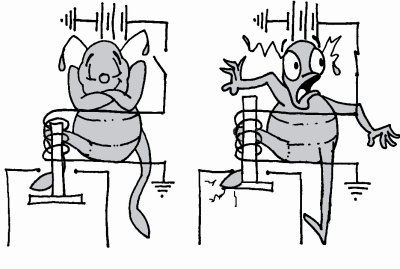
\includegraphics[scale=0.5]{fig-sets/bugcerto.png}
\end{wrapfigure}
The first computer was\index{Konrad Zuse!Ursula Walk} 
constructed\index{Konrad Zuse!first computer}
by Konrad Zuse,\index{Zuse}\index{Konrad Zuse}
a German civil engineer, and his assistant,
Ms. Ursula Walk,\index{Ursula Hebekeuser} née Hebekeuser.
The first computers, like those of Zuse and Walk,
were based on relays.\index{Konrad Zuse!relays}
These are
bulky electrical devices, typically incorporating
an electromagnet, which is activated by a current
in one circuit to turn on or off another circuit.
Computers made of such a contrivance were enormous,
slow, and unreliable. Therefore, on September 9th, 1945,
a moth flew into one of the relays of the Harvard  Mark II
computer and jammed it. From that time on,   {\em bug}
became the standard word to indicate
an error that prevents a computer from working as intended.

Due to bugs, compilers of languages like Clean
and Haskell frequently return error messages,
instead of generating code and running the
corresponding programs. The Steel Bank Common Lisp language
does not interrupt code generation when the
compiler spots a bug, all the same
it does issue warnings
that help find the problem before the embarassment
of failure being manifest on the client's terminal.
Scheme does not possess such a kind of oracular
compiler. It report errors only when you execute
the code.


\section{Missing parenthesis}\index{Bugs!missing parenthesis}
There is only one kind of bug that scheme
reports at compile
time: missing parenthesis.
This bug  is annoying, because the compiler
does not  report its position accurately.
For example, try to compile the code of Listing~\ref{missing-semiColon}.
The compiler issues the
following error message:
\begin{quote}
\begin{verbatim}
File "src/manydefs.scm", line 12, character 159:
#(define (fn+1 n fn fn-1)
#^
*** ERROR:read
Unexpected end-of-file -- Unclosed list
    1. load, src/manydefs.scm:8
\end{verbatim}
\end{quote}
The error is on line 15, where a right parenthesis is missing.
However,  the error message is misleading,
as it points to the wrong line and does not mention
the parenthesis.

Whenever you receive a message
of `unexpected end-of-file', my advice is to
look for a missing parenthesis.


\begin{figure}[!h]\index{define}
\begin{fmpage}{0.8\textwidth}
\begin{verbatim}
;; File: fvalue.scm

(define  (future-value pv i n)
(* (expt (+ (/ i 100.0 1) n) 
   pv))
);;end define

(define (fat n)
(if (< n 1) 1
 (* (fat (- n 1)) n)))

(define (fn+1 n fn fn-1)
(if (< n 2) fn
 (fn+1 (- n 1
       (+ fn fn-1) fn)))

(define (quick xs)
(if (null? xs) xs
(append
    (quick (filter (lambda(x) (< x (car xs)))
                   (cdr xs)))
    (list (car xs))
    (quick (filter (lambda(x) (>= x (car xs)))
                   (cdr xs))) )))
\end{verbatim}
\end{fmpage}

\begin{fmpage}{0.8\textwidth}
\begin{verbatim}
1:=> (load "src/manydefs.scm")
File "src/manydefs.scm", line 12, character 159:
#(define (fn+1 n fn fn-1)
#^
*** ERROR:read
Unexpected end-of-file -- Unclosed list
\end{verbatim}
\end{fmpage}
\caption{Future Value Program}
\label{missing-semiColon}
\end{figure}


\chapter{Finite Automaton}
\index{Finite automata}\label{chap:finite-automaton}
A deterministic finite automaton
is a finite state machine that accepts or rejects
finite strings of chars and only produces
a unique computation  for each input string.
Figure~\ref{fig:automaton} below illustrates a deterministic
finite automaton using a state diagram.
The aforementioned automaton recognizes words
and puctuation marks from a text using
the Roman alphabet, which is the same
as in English. Therefore,
this automaton can  accept a
stream of words and punctuation from an English text.

\begin{figure}[!h]
\renewcommand\figurename{Fig.}
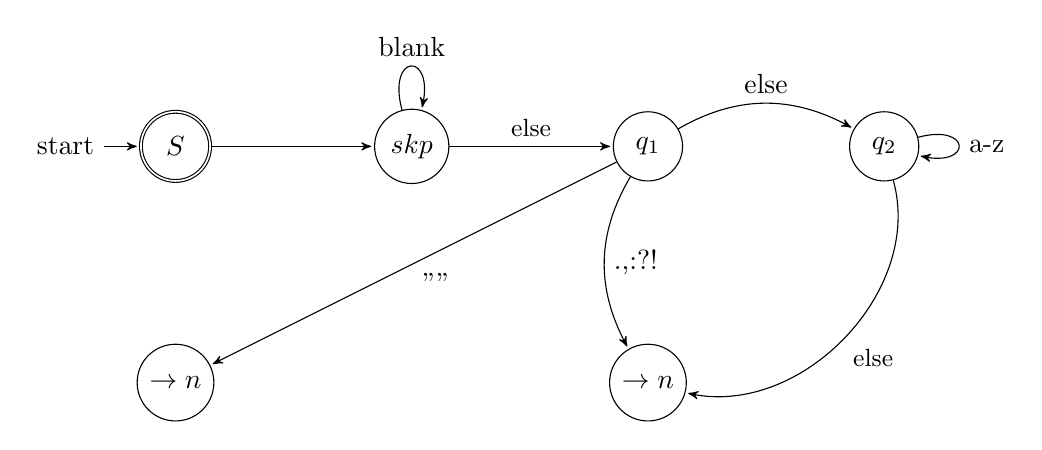
\begin{tikzpicture}[>=stealth',shorten >=1pt,on grid,
                   auto,node distance=3cm]
\node[initial,state,accepting] (S)      {$S$};
\node[state]         (q0) [right of=S]  {$skp$};
\node[state]         (q1) [right of=q0]  {$q_1$};
\node[state]         (q3) [right of=q1] {$q_2$};
\node[state]         (r0) [below of= S] {$\rightarrow n$};
\node[state]         (q2) [below of=q1] {$\rightarrow n$};

\path[->] (S)  edge  (q0)
(q0) edge [->] node {\small else} (q1)
(q1) edge [bend right] node {.,:?!} (q2)
(q0) edge [loop above] node {blank} (q0)
(q3) edge [bend left=60] node {\small else} (q2)
(q1) edge [->,bend left] node {else} (q3)
(q1) edge [] node {""} (r0);
\path[->]
(q3) edge [loop right] node {a-z} (q3);
\end{tikzpicture}
\caption{Finite automaton that recognizes English words}
\label{fig:automaton}
\end{figure}

In the automaton of figure~\ref{fig:automaton}, there
are three states: $skp$, $q_1$ and $q_2$.
The automaton remains in the state $skp$ as long as
the stream produces blank chars, i. e., \verb|#\space|,
\verb|#\newline| or \verb|#\tab|. If the computation
reaches the end of the string, the automaton  stops.
If a punctuation mark appears
in the stream, the automaton accepts it, and 
returns $\rightarrow n$. If the  $q_1$ state
receives an alphabetical letter, the automaton
goes to state $q_2$ and remains there 
as long as the reader keeps feeding letters.
\index{String!string.find}
\index{String!strings-ref}
\index{String!string-length}
\index{String!string}


\begin{figure}[!h]
\begin{fmpage}{0.9\linewidth}
\begin{verbatim}
(define (end? s n) (<= (string-length s) n))

(define (pct? s n)
   (string-char-index ".,?" (string-ref s n)))

(define (blk? s n)
   (string-char-index " \n" (string-ref s n)))

(define (letter? s n)
  (and (not (pct? s n)) (not (blk? s n)) ))

(define (skp n s)
   (if (or (end? s n) (not (blk? s n))) n
      (skp (+ n 1) s)))

(define (q1 n s)
   (cond ( (end? s n) n)
         ( (pct? s n) (+ n 1) )
         (else (q3 n s)) ))

(define (q3 n s )
   (cond ( (end? s n) n)
         ( (letter?  s n) (q3 (+ n 1) s))
         (else  n)))

(define (tkz s #!optional (n 0) 
                          (i (skp n s))
                          (j (q1 i s)))
  (cond ( (end? s i) '())
          ( (end? s j) (list (substring s i j)))
          (else (cons (substring s i j) (tkz s j)) ) ))

\end{verbatim}
\end{fmpage}
\caption{Finite Automaton in Scheme}
\label{FA-in-Scheme}
\end{figure}

\begin{verbatim}
1:=> (load "src/auto-one.scm")
src/auto-one.scm
1:=> (tkz "She walks in beauty, like the night")
(She walks in beauty , like the night)
\end{verbatim}


\begin{thebibliography}{99}


\bibitem{Abelson} Harold Abelson, Gerald Jay Sussman and
Julie Sussman. Structure and Interpretation of
Computer Programs. The MIT Press, Second Edition, 1996.

\bibitem{Felleisen} Matthias Felleisen,
Robert Bruce Findler, Matthew Flatt, Shriram Krishnamurthi.
How to Design Programs.
Available from \verb|http://www.htdp.org|

\bibitem{Sitaram} Dorai Sitaram. Teach yourself Scheme
in Fixnum Days. Available
from \verb|http://ds26gte.github.io/tyscheme/|

\bibitem{Hoyte} Doug Hoyte. Let Over Lambda. Hoytech, 2008. ISBN: 978-1-4357-1275-1

\bibitem{Church1932} A. Church, A set of postulates for the foundation of logic, Annals of Mathematics, Series 2, 33:346–366 (1932).

\bibitem{Church} Alonzo Church. The Calculi of Lambda Conversion. Princepton University Press, 1986.

\bibitem{Dybvig} R. Kent Dybvig. The Scheme Programming Language.
Available from \verb|http://www.scheme.com/tspl4/|

\end{thebibliography}

\printindex

\end{document}

\frontmatter

\chapter*{Preface}

Femto is a tiny Emacs clone,
originally derived from a minimalist
editor called Atto. Although built
upon the C Atto codebase, Femto can
be customized using the Scheme dialect.

The fundamental paradigm of Emacs is that it
rests on a small core, but can be
extended and customized through
the Lisp programming language.

Istead of requiring from the programmer a compile,
build, test and fix cycle ---
Lisp offers a Read, Eval, Print Loop (REPL).
\begin{enumerate}
\item {\bf Read.} The REPL reads
a symbolic expression 
such as \verb|(+ 42 13 4)| from
a text terminal. The symbolic expression -- sexpr --
always has the form: $(\textrm{operation}\;a_1\;a_2\ldots a_n)$,
where $a_1$, $a_2$\ldots $a_n$ are the arguments of
the operation.
\item {\bf Eval.} The compiler translates the symbolic
expression to machine language, then executes the
generated code and calculates the corresponding
value.
\item {\bf Print.} The value produced in step 2 is printed.
\item {\bf Loop.} The REPL returns to step 1.
\end{enumerate}

Since Lisp is usually compiled, it is
much faster than interpreted languages.
However, to facilitate portability,
scheme does not generate
native code, but compiles symbolic expressions
to a virtual machine language. As a consequence of
this choice, scheme is not as fast as other
Lisp dialects, such as sbcl and Racket. Notwithstanding,
it is about four times faster than Python
and forty times faster than Tiny Scheme.

The REPL approach enables fast prototyping
of extensions as each idea can be tested
individually on the command line inside
the editor with an immediate result check.

For historical reasons, the reference GNU
Emacs implementation uses a specialised version of
lisp known as Emacs Lisp.  However, the Emacs Lisp
dialect is not standard lisp, being used
only by the GNU Emacs editor and its
derivatives.

Lisp was chosen
as the extension language
for Emacs for the following reasons:
\begin{enumerate}
\item Lisp is open source.
\item Lisp is small and written in C.
\item After loading the \verb|r5rs.scm| library
provided in the emacs distribution,
the user can bridge the syntactic gap
between Bigloo and R5RS Scheme.
In the majority of situations, the \verb|r5rs.scm|
library is compatible
with the standard Scheme dialect. This means that
one can use classical Scheme tutorials to learn
how to configure and customize emacs.
The Structure and Interpretation of Computer Programs
is the most popular of these tutorials.
Of course, you can use the content of the
present text to the same effect.
\item Scheme is fast.
\end{enumerate}    


